\documentclass[sigconf,screen]{acmart}
\pdfoutput=1

% %%%%%%%%%%%%%%%%%%%%%%%%
% %Hack to remove some irrelevant copyright info.
% \settopmatter{printacmref=false} % Removes citation information below abstract
% \renewcommand\footnotetextcopyrightpermission[1]{} % removes footnote with conference information in first column
% \pagestyle{plain} % removes running headers

% \setlength{\headheight}{27pt} 
% \setlength{\footskip}{14pt}

% \makeatletter
% \renewcommand\@formatdoi[1]{\ignorespaces}
% \makeatother
% %%%%%%%%%%%%%%%%%%%%%%%%

\usepackage{natbib}
\usepackage{algorithm}
\usepackage[noend]{algorithmic}
\usepackage{amsmath}
\usepackage{geometry}
\usepackage{verbatim}
\usepackage{tabularx}
\usepackage{graphicx}
\usepackage{amsfonts}
\usepackage{cleveref}
\usepackage{multirow}
\usepackage{microtype}
\usepackage{enumitem}
\usepackage{xcolor}
\usepackage{hyperref}
%\usepackage[
% subtle
 %moderate
%]{savetrees}
%\usepackage{blindtext}
\hypersetup{
    colorlinks=true,
    linkcolor=blue,
    filecolor=magenta,      
    urlcolor=cyan,
    citecolor=orange,
}
\urlstyle{same}
\usepackage{flushend}

%\usepackage{biblatex}
%\DeclareMathSizes{10}{9}{6}{5}
\newtheorem*{theorem*}{Theorem}
\newtheorem{theorem}{Theorem}[section]
\newtheorem{corollary}[theorem]{Corollary}
\newtheorem{lemma}[theorem]{Lemma}
\newtheorem{proposition}{Proposition}[section]
\newtheorem{claim}{Claim}[section]
\newtheorem{definition}{Definition}[section]
\newtheorem{remark}{Remark}[section]
\newtheorem{observation}{Observation}[section]
\newtheorem{condition}{Condition}[section]

\DeclareMathOperator*{\argmax}{arg\,max}
\DeclareMathOperator*{\argmin}{arg\,min}

\newcommand{\INPUT}{\item[{\bf Input:}]}
\newcommand{\OUTPUT}{\item[{\bf Output:}]}

\newcommand{\partdiff}[2]{\frac{\partial {#1}}{\partial {#2}}}
\newcommand{\secdiff}[2]{\frac{\partial^2 {#1}}{\partial {#2}^2}}
\newcommand{\mixdiff}[3]{\frac{\partial^2 {#1}}{{\partial {#2}}{\partial {#3}}}}
\newcommand{\iprod}[2]{\left\langle {#1}, 
{#2} \right \rangle}
\newcommand{\etal}{et al.\ }
\newcommand{\ceil}[1]{\lceil #1 \rceil}
\newcommand{\floor}[1]{\lfloor #1 \rfloor}
\newcommand{\bigfloor}[1]{\left\lfloor #1 \right\rfloor}
\newcommand{\bigceil}[1]{\left\lceil #1 \right\rceil}
\newcommand{\eps}{\varepsilon}
\newcommand{\E}{\mathbf{E}}
\newcommand{\Var}{\mathbf{Var}}
\newcommand{\poly}{\mathrm{poly}}
\newcommand{\rank}{\mathrm{rank}}
\newcommand{\tr}[1]{\mathrm{Tr}\left( #1 \right)}

\newcommand{\cA}{\mathcal{A}}
\newcommand{\cI}{\mathcal{I}}
\newcommand{\cM}{\mathcal{M}}
\newcommand{\cF}{\mathcal{F}}
\newcommand{\cD}{\mathcal{D}}
\newcommand{\cP}{\mathcal{P}}
\newcommand{\cE}{{\mathcal{E}}}
\newcommand{\cX}{\mathcal{X}}
\newcommand{\cH}{{\mathcal{H}}}
\newcommand{\cR}{\mathcal{R}}
\newcommand{\cB}{\mathcal{B}}
\newcommand{\cQ}{\mathcal{Q}}
\newcommand{\cZ}{\mathcal{Z}}
\newcommand{\cS}{\mathcal{S}}
\newcommand{\RR}{{\mathbb R}}
\newcommand{\ZZ}{{\mathbb Z}}
\newcommand{\NN}{{\mathbb N}}
\newcommand{\id}[1]{\mathbbm{1}_{#1}}

\newcommand{\vx}{\mathbf{x}}
\newcommand{\vy}{\mathbf{y}}
\newcommand{\xdot}{\dot \vx}
\newcommand{\ydot}{\dot \vy}
\newcommand{\dt}{\mathrm{d}t}
\newcommand{\dx}{\mathrm{d}x}
\newcommand{\dF}{\mathrm{d}F}
\newcommand{\ddp}{\frac{\mathrm{d}}{\mathrm{d}p}}

%\newcommand{\qed}{\hfill{\rule{2mm}{2mm}}}

\def\b1{{\bf 1}}
\def\be{{\bf e}}
\def\ba{{\bf a}}
\def\bg{{\bf g}}
\def\bX{{\bf X}}
\def\bb{{\bf b}}
\def\bc{{\bf c}}
\def\bx{{\bf x}}
\def\by{{\bf y}}
\def\bv{{\bf v}}
\def\bV{{\bf V}}
\def\bw{{\bf w}}
\def\bz{{\bf z}}
\def\tx{\tilde{\bf x}}

\newcommand{\paul}[1]{{\color{blue} [[PAUL: #1]]}}
\newcommand{\aram}[1]{{\color{violet} [[ARAM: #1]]}}
\DeclareMathOperator\sech{sech}
\DeclareMathOperator\erf{erf}

\title{Elo-MMR: A Rating System for Massive Multiplayer Competitions}

%\title{An Elo-like System for Massive Multiplayer Competitions}

\author{Aram Ebtekar}
\affiliation{%
  %unaffiliated: \institution{University of British Columbia}
  \city{Vancouver}
  \state{BC}
  \country{Canada}
}
\email{aramebtech@gmail.com}

\author{Paul Liu}
\affiliation{%
  \institution{Stanford University}
  \city{Stanford}
  \state{CA}
  \country{USA}
}
\email{paul.liu@stanford.edu}

\copyrightyear{2021}
\acmYear{2021}
\setcopyright{iw3c2w3}
\acmConference[WWW '21]{Proceedings of the Web Conference 2021}{April 19--23, 2021}{Ljubljana, Slovenia}
\acmBooktitle{Proceedings of the Web Conference 2021 (WWW '21), April 19--23, 2021, Ljubljana, Slovenia}
\acmPrice{}
\acmDOI{10.1145/3442381.3450091}
\acmISBN{978-1-4503-8312-7/21/04}

\settopmatter{printacmref=true}

\begin{CCSXML}
<ccs2012>
<concept>
<concept_id>10002951.10003317.10003338.10003343</concept_id>
<concept_desc>Information systems~Learning to rank</concept_desc>
<concept_significance>500</concept_significance>
</concept>
<concept>
<concept_id>10010147.10010257.10010293.10010300</concept_id>
<concept_desc>Computing methodologies~Learning in probabilistic graphical models</concept_desc>
<concept_significance>500</concept_significance>
</concept>
</ccs2012>
\end{CCSXML}

\ccsdesc[500]{Information systems~Learning to rank}
\ccsdesc[500]{Computing me-thodologies~Learning in probabilistic graphical models}

\keywords{rating system, skill estimation, mechanism design, competition, bayesian inference, robust, incentive-compatible, elo, glicko, trueskill}

\begin{document}

%\everypar{\looseness=-1}
\linepenalty=200

\begin{abstract}
Skill estimation mechanisms, colloquially known as rating systems, play an important role in competitive sports and games. They provide a measure of player skill, which incentivizes competitive performances and enables balanced match-ups. In this paper, we present a novel Bayesian rating system for contests with many participants. It is widely applicable to competition formats with discrete ranked matches, such as online programming competitions, obstacle courses races, and video games. The system's simplicity allows us to prove theoretical bounds on its robustness and runtime. In addition, we show that it is \emph{incentive-compatible}: a player who seeks to maximize their rating will never want to underperform. Experimentally, the rating system surpasses existing systems in prediction accuracy, and computes faster than existing systems by up to an order of magnitude.
\end{abstract}

\maketitle
% \pagestyle{plain}


\section{Introduction}

% \begin{comment}
% Notes to self:
% - Should we do all-pairs ELO/Glicko per contest as a comparison?
%     - Performances where you do really well is amplified (\#1 is treated as O(n) wins where n is the number of competitors)
% - Can we prove the "aligned incentives" property? I.e. is a participant ever incentivized to lose?
%     - Can show that edits to past performance is monotonic w.r.t. to the edits

% Important points in introduction:
% - Rating systems are ad-hoc, preferences for algorithms based mostly on word-of-mouth and first movers.
% - Different domains use different systems (chess, football, etc --> elo based. team-based online games --> trueskill based or glicko based. coding contests --> ad-hoc, codeforces)
% - In general, the more complicated the rating system, the less adoptation.
% - Players overwhelmingly prefer the ability to understand and predict their own performance.
% - Rating systems are even used outside of sports: "Web-scale bayesian clickthrough
% rate prediction for sponsored search advertising in microsoft’s bing search
% engine" pits ads against each other in a TrueSkill-like fashion.
% - The goal of a rating system is two-fold: firstly to predict the results between players, but also equally as important is to give the players an easily interpretable proxy for their skill.

% Brief literature review:
% - In programming contests the actual scores do not matter much, the ranks give the most discriminative information
% - Talk about area of pairwise comparisons
%     - Paired comparisons assume static "ability" throughout time.
%     - First to look at time-varying paired comparisons was the glicko rating system
% - Glicko and Glicko 2:
%     - Improvement upon Elo in that the deviation was also explicitly modelled
%     - A drift parameter was also added to increase rating volatility over time
%     - This in turn increases the rating uncertainty since the uncertainty is updated from the volatility
%     - Flaws famously exploited in pokemon go, as rating gain is proportional to rating uncertainty
% - MOV Elo techniques:
%     - These not only take in ranking as input, but also "margin of victory". This is appropriate for more fine-grained contests where the same type of contest is played over and over again (e.g. tennis). For programming contests this is not as useful since the contest changes over and over again. Methods not directly applicable in our setting.
%     - Streamlines interface between rating system and contest type and for contest authors. More applicable to other domains. Goodhart's Law.
% - IRT rating system:
%     - Tasks of a contest are modelled explicitly. Allows for more fine grained predictions (such as the number of problems solved during a contest)
% - WHR (Who-Rating-History): a bayesian approach to ratings that takes into account time-varying strength
%     - Three types of rating sys: Static, Incremental, Decayed-History
%     - Our rating system is Incremental. Inferior in the following sense: suppose that there are two players (A & B) that only play against each other. Then A plays against established players. This gives information to B's rating, but incremental systems leave B's rating unchanged.
%     - This rating system doesnt seem to necessarily have a monotonicity property: the addition of a game could decrease the ratings of some of the players in the system who do not directly participate in the game? Players are not typically happy about this; good motivation for our second algorithm property
%     - Limit of large # of players guarantee a connectivity property
% - TrueSkill and TrueSkill 2: 
%     - Models games where medium sized teams of players play against each other
%     - Each user has some skill drawn from a distribution
%     - The performance on any given day is drawn from a distribution centred at the skill
%     - The performance of a team is the sum of team skills
%     - A parameter eps is defined so that performances with difference less than eps is counted as a tie.
%     - Trained through message passing
%     - Used in massive scale in Halo 2
%     - Convergence properties unclear, hard to proof stuff about it
%     - Normal vs logistics support.
%     - TrueSkill 2 takes into account further application-specific statistics
% - Trueskill Through Time:
%     - Similar to WHR in that a new game affects whole history. Does this suffer from non-monotonicity?
% - TrueSkill StPb:
%     - Improved on trueskill by adapting factor graph to handle ties in a principled way
%     - Nodes are added to the factor graph grouping teams that are tied
%     - Instead of summing team performances, non-linear team performance functions are explored
% - TeamSkill and TeamSkill Evolved:
%     - An ensemble learner that leverages TrueSkill, Elo, and Glicko to better predict ratings in the presence of "team chemistry" and non-equal team sizes.
%     - However only works when teams play together semi-consistently
% - Codeforces & leetcode:
%     - Generalized Elo system
%     - Heuristics to fight against inflation
%     - O(n^2) time.
%     - Used in leetcode as well, somewhat of an industry standard
%     - total website use at least 3 million users
% - Topcoder:
%     - More similar to glicko in the sense that each user has a rating deviation
%     - Successfully attacked by Forisek

% The Elo rating system assigns a quantitative measure of skill to each player. For example, an average player may be rated 1500, while a top player may exceed 2500. The scale is arbitrary, but can be used to rank players relative to one another. The odds of any one player winning against another may be estimated from the difference in their ratings. The famous Elo system, and variants such as Glicko \cite{G99}, provide useful formulas for updating ratings of players who compete 1v1 against one another, resulting in a winner and a loser. These algorithms have some nice properties: they are fairly simple, fast, and only modify the ratings of the two participating players.

% Now let's consider a general setting in which a typical contest has much more than two participants. An arbitrary number of players compete simultaneously at a task. Rather than producing just a winner and a loser, the contest ranks its participants 1st place, 2nd, 3rd, and so on. This description fits popular programming competition websites such as Codeforces \cite{Codeforces} and Topcoder \cite{Topcoder}, each of which has tens of thousands of rated members from across the globe. Each publishes its own rating system, but without much theoretical justification to accompany the derivations.

% We build Elo-MMR upon a more rigorous probabilistic model, mirroring the Bayesian development of the Glicko system. In doing so, we inherit its nice properties in practice, resolving known issues with the Codeforces and Topcoder systems. Compared with these systems, it achieves faster convergence and robustness against unusual performances. Issues specific to Codeforces than we improve upon are the overall spread of ratings, inter-division boundary artifacts, and inflation (TODO: cite, and quantify this with tests). An issue specific to Topcoder that we eliminate completely is non-monotonicity: simply put, there are cases in which improving a member's past performance would actually decrease their Topcoder rating, and vice-versa \cite{forivsektheoretical}.

% Furthermore, Elo-MMR retains simplicity and efficiency on par with the other systems. To demonstrate this, I provide a very efficient parallel implementation that can process the entire history of rated competitions hosted by Codeforces on a modest quad-core laptop within 30 minutes. It is implemented entirely within the safe subset of Rust using the Rayon crate; hence, the Rust compiler verifies that it contains no data races.

% This paper is organized as follows: in section 2, we develop a Bayesian model for the competitions. Rating updates are phrased as a latent skill estimation problem, which is naturally divided into two phases. Sections 3 and 4 describe each of these phases in turn, and supplement the derivations with some intuitive interpretations. Then in section 5, we discuss some ways to model uncertainty, in a manner analogous to the Glicko system. In section 6, we discuss some properties of the Elo-MMR system in comparison with the Codeforces and Topcoder systems. Finally, section 7 presents the conclusions of this work.
% \end{comment}

Competitions, in the form of sports, games, and examinations, have been with us since antiquity. Many competitions grade performances along a numerical scale, such as a score on a test or a completion time in a race. In the case of a college admissions exam or a track race, scores are standardized so that a given score on two different occasions carries the same meaning. However, in events that feature novelty, subjectivity, or close interaction, standardization is difficult. The Spartan Races, completed by millions of runners, feature a variety of obstacles placed on hiking trails around the world~\cite{Spartan}. Rock climbing, a sport to be added to the 2020 Olympics, likewise has routes set specifically for each competition. DanceSport, gymnastics, and figure skating competitions have a panel of judges who rank contestants against one another; these subjective scores are known to be noisy~\cite{DanceSport}. 
%Most board games feature considerable inter-player interaction.
In all these cases, scores can only be used to compare and rank participants at the same event. Players, spectators, and contest organizers who are interested in comparing players' skill levels across different competitions will need to aggregate the entire history of such rankings. A strong player, then, is one who consistently wins against weaker players. To quantify skill, we need a \textbf{rating system}.


Good rating systems are difficult to create, as they must balance several mutually constraining objectives. First and foremost, rating systems must be accurate, in that ratings provide useful predictors of contest outcomes. Second, the ratings must be efficient to compute: within video game applications, rating systems are predominantly used for matchmaking in massively multiplayer online games (such as Halo, CounterStrike, League of Legends, etc.)~\cite{HMG06, MCZ18, Y14}. These games have hundreds of millions of players playing tens of millions of games per day, necessitating certain latency and memory requirements for the rating system~\cite{AL09}. Third, rating systems must be \textbf{incentive-compatible}: a player's rating should never increase had they scored worse, and never decrease had they scored better.
%should never depend inversely on an absolute score. 
This is to prevent players from regretting a win, or from throwing matches to game the system. Rating systems that can be gamed often create disastrous consequences to player-base, potentially leading to the loss of players~\cite{pokemongo}. Finally, the ratings provided by the system must be human-interpretable: ratings are typically represented to players as a single number encapsulating their overall skill, and many players want to understand and predict how their performances affect their rating~\cite{G95}.

% Should we consider something about robustness, and about ratings not changing when a player doesn't compete? There are two things that these systems have in common. First, all of the these systems propagate changes forward in time, never backward. This is a strict requirement of the system in most cases, as users prefer their historical ratings to state fixed (even if it's possible to infer more accurate historical ratings from future matches). Such a property will be a requirement of our system as well.

Classically, rating systems were designed for two-player games. The famous Elo system~\cite{E61}, as well as its Bayesian successors Glicko and Glicko-2, have been widely applied to games such as Chess and Go~\cite{G95, G99, G12}. Both Glicko versions model each player's skill as a real random variable that evolves with time according to Brownian motion. Inference is done by entering these variables into the Bradley-Terry model~\cite{BT52}, which predicts probabilities of game outcomes. Glicko-2 refines the Glicko system by adding a rating volatility parameter. Unfortunately, Glicko-2 is known to be flawed in practice, potentially incentivizing players to lose in what's known as ``volatility farming''. In some cases, these attacks can inflate a user's rating \emph{several hundred points} above its natural value, producing ratings that are essentially impossible to beat via honest play. This was most notably exploited in the popular game of Pokemon Go~\cite{pokemongo}. See \Cref{sec:mono} for a discussion of this issue, as well as an application of this attack to the Topcoder rating system.

The family of Elo-like methods just described only utilize the binary outcome of a match. In settings where a scoring system provides a more fine-grained measure of match performance, Kovalchik~\cite{K20} has shown variants of Elo that are able to take advantage of score information. For competitions consisting of several set tasks, such as academic olympiads, Fori{\v{s}}ek~\cite{forivsektheoretical} developed a model in which each task gives a different ``response'' to the player: the total response then predicts match outcomes. However, such systems are often highly application-dependent and hard to calibrate.

%In terms of predictive power, the main disadvantage of Elo-like methods is that they are ``history-less'' and ``static''. That is, previous competitions of an individual are forgotten and summarized solely through a few per-user parameters. Consider an example where two groups of users compete within their own groups and never outside of their group. To compare the two groups, we may choose a representative user from each group to compete against each other. Given the results of this match, it should be possible to calibrate the ratings of all the users in the two groups accordingly. However, Elo-like methods only update the ratings of the two users participating in the match. Coulom~\cite{C08} exploit this observation by retaining the entire match history of a user, allowing for more accurate predictions. 

Though Elo-like systems are widely used in two-player settings, one needn't look far to find competitions that involve much more than two players. In response to the popularity of team-based games such as CounterStrike and Halo, many recent works focus on competitions that are between two teams~\cite{HLW06, CJ16, LCFHH18, GFYLWTFC20}. Another popular setting is many-player contests such as academic olympiads: notably, programming contest platforms such as Codeforces, Topcoder, and Kaggle~\cite{Codeforces, Topcoder, Kaggle}. As with the aforementioned Spartan races, a typical event attracts thousands of contestants. Programming contest platforms have seen exponential growth over the past decade, collectively boasting millions of users~\cite{KaggleMilestone}. As an example, Codeforces gained over 200K new users in 2019 alone~\cite{CFResults}.
%but they do not present efficient extensions for settings in which players are sorted into more than two, let alone thousands, of distinct places. For these cases, a rating system must take in a final ranking of the competitors, and produce a list of rating updates. 

In ``free-for-all'' settings, where $N$ players are ranked individually, the Bayesian Approximation Ranking (BAR) algorithm~\cite{WL11} models the competition as a series of $\binom N2$ independent two-player contests. In reality, of course, the pairwise match outcomes are far from independent. Thus, TrueSkill~\cite{HMG06} and its variants~\cite{NS10, DHMG07, MCZ18} model a player's performance during each contest as a single random variable. The overall rankings are assumed to reveal the total order among these hidden performance variables, with various methods used to model ties and teams. For a textbook treatment of these methods, see~\cite{Winn19}. These rating systems are efficient in practice, successfully rating userbases that number well into the millions (the Halo series, for example, has over 60 million sales since 2001~\cite{Halo}).

The main disadvantage of TrueSkill is its complexity: originally developed by Microsoft for the popular Halo video game, TrueSkill performs approximate belief propagation, which consists of message passing on a factor graph, iterated until convergence. Aside from being less human-interpretable, this complexity means that, to our knowledge, there are no proofs of key properties such as runtime and incentive-compatibility. Even when these properties are discussed~\cite{MCZ18}, no rigorous justification is provided. In addition, we are not aware of any work that extends TrueSkill to non-Gaussian performance models, which might be desirable to limit the influence of outlier performances (see \Cref{sec:robust}).

It might be for these reasons that popular platforms such as Codeforces and Topcoder opted for their own custom rating systems. These systems are not published in academia and do not come with Bayesian justifications. However, they retain the formulaic simplicity of Elo and Glicko, extending them to settings with much more than two players. The Codeforces system includes ad hoc heuristics to distinguish top players, while curbing rampant inflation. Topcoder's formulas are more principled from a statistical perspective; however, it has a volatility parameter similar to Glicko-2, and hence suffers from similar exploits~\cite{forivsektheoretical}. Despite their flaws, these systems have been in place for over a decade, and have more recently gained adoption by additional platforms such as CodeChef and LeetCode~\cite{LeetCode, CodeChef}.


\paragraph{Our contributions} 
In this paper, we describe the Elo-MMR rating system, obtained by a principled approximation of a Bayesian model similar to Glicko and TrueSkill. It is fast, embarrassingly parallel, and makes accurate predictions. Most interesting of all, its simplicity allows us to rigorously analyze its properties: the ``MMR'' in the name stands for ``Massive'', ``Monotonic'', and ``Robust''. ``Massive'' means that it supports any number of players with a runtime that scales linearly; ``monotonic'' is a synonym for incentive-compatible, ensuring that a rating-maximizing player always wants to perform well; ``robust'' means that rating changes are bounded, with the bound being smaller for more consistent players than for volatile players. Robustness turns out to be a natural byproduct of accurately modeling performances with heavy-tailed distributions, such as the logistic. TrueSkill is believed to satisfy the first two properties, albeit without proof, but fails robustness. Codeforces only satisfies incentive-compatibility, and Topcoder only satisfies robustness.

Experimentally, we show that Elo-MMR achieves state-of-the-art performance in terms of both prediction accuracy and runtime on industry datasets. In particular, we process the entire Codeforces database of over 300K rated users and 1000 contests in well under a minute, beating the existing Codeforces system by an order of magnitude while improving upon its accuracy. Furthermore, we show that the well-known Topcoder system is severely vulnerable to volatility farming, whereas Elo-MMR is immune to such attacks. A difficulty we faced was the scarcity of efficient open-source rating system implementations. In an effort to aid researchers and practitioners alike, we provide open-source implementations of all rating systems, dataset mining, and additional processing used in our experiments at {\tt\url{https://github.com/EbTech/Elo-MMR}}.

\paragraph{Organization}
In \Cref{sec:bayes_model}, we formalize the details of our Bayesian model. We then show how to estimate player skill under this model in \Cref{sec:main-alg}, and develop some intuitions of the resulting formulas. As a further refinement, \Cref{sec:skill-drift} models skill evolutions from players training or atrophying between competitions. This modeling is quite tricky as we choose to retain players' momentum while preserving incentive-compatibility. While our modeling and derivations occupy multiple sections, the system itself is succinctly presented in \Cref{alg:main,alg:diffuse,alg:update}. In \Cref{sec:properties}, we perform a volatility farming attack on the Topcoder system and prove that, in contrast, Elo-MMR satisfies several salient properties, the most critical of which is incentive-compatibility. Finally, in \Cref{sec:experiments}, we present experimental evaluations, showing improvements over industry standards in both accuracy and speed. An extended version of this paper, with additional proofs and experiments, can be found at {\tt\url{https://arxiv.org/abs/2101.00400}}.

\section{A Bayesian Model for Massive Competitions}
\label{sec:bayes_model}
% The method is best-suited for competitions in which the most pertinent information is round rankings. Note that, in the programming contest setting, this means we discard specific information about player scores, which are difficult to model and depend heavily on the specifics of the problem set. This method would be ill-suited to model, for instance, track races, where a runner's absolute time is more informative than relative rankings. On the other hand, it may be very well-suited to obstacle-course races, if each round consists of novel obstacles that make the absolute times hard to interpret.

We now describe the setting formally, denoting random variables by capital letters. A series of competitive \textbf{rounds}, indexed by $t=1,2,3,\ldots$, take place sequentially in time. Each round has a set of participating \textbf{players} $\cP_t$, which may in general overlap between rounds. A player's \textbf{skill} is likely to change with time, so we represent the skill of player $i$ at time $t$ by a real random variable $S_{i,t}$.

In round $t$, each player $i\in \cP_t$ competes at some \textbf{performance} level $P_{i,t}$, typically close to their current skill $S_{i,t}$. The deviations $\{P_{i,t}-S_{i,t}\}_{i\in\cP_t}$ are assumed to be i.i.d. and independent of $\{S_{i,t}\}_{i\in\cP_t}$.

Performances are not observed directly; instead, a ranking gives the relative order among all performances $\{P_{i,t}\}_{i\in\cP_t}$. In particular, ties are modelled to occur when performances are exactly equal, a zero-probability event when their distributions are continuous.\footnote{
%If $e$ contains ties, then $(E_t = e)$ has probability zero in our model. 
The relevant limiting procedure is to treat performances within $\epsilon$-width buckets as ties, and letting $\epsilon\rightarrow 0$. This technicality appears in the proof of \Cref{thm:uniq-max}.} This ranking constitutes the observational \textbf{evidence} $E_t$ for our Bayesian updates. The rating system seeks to estimate the skill $S_{i,t}$ of every player at the present time $t$, given the historical round rankings $E_{\le t} := \{ E_1,\ldots,E_t \}$.

We overload the notation $\Pr$ for both probabilities and probability densities: the latter interpretation applies to zero-probability events, such as in $\Pr(S_{i,t} = s)$. We also use colons as shorthand for collections of variables differing only in a subscript: for instance, $P_{:,t}:=\{P_{i,t}\}_{i\in\cP_t}$. The joint distribution described by our Bayesian model factorizes as follows:
\begin{align}
    &\Pr(S_{:,:}, P_{:,:}, E_:) \label{eq:model}
    \\&= \prod_i \Pr(S_{i,0})
    \prod_{i,t} \Pr(S_{i,t}\mid S_{i,t-1})
    \prod_{i,t} \Pr(P_{i,t}\mid S_{i,t})
    \prod_t \Pr(E_t\mid P_{:,t}), \nonumber
\end{align}
\vspace{-1.5em}
\begin{align*}
    \text{where } \Pr(S_{i,0}) &\text{ is the initial skill prior,}
    \\\Pr(S_{i,t}\mid S_{i,t-1}) &\text{ is the skill evolution model (\Cref{sec:skill-drift}),}
    \\\Pr(P_{i,t}\mid S_{i,t}) &\text{ is the performance model, and}
    \\\Pr(E_t\mid P_{:,t}) &\text{ is the evidence model.}
\end{align*}
For the first three factors, we will specify log-concave distributions (see \Cref{def:log-concave}). The evidence model, on the other hand, is a deterministic indicator. It equals one when $E_t$ is consistent with the relative ordering among $\{P_{i,t}\}_{i\in\cP_t}$, and zero otherwise.

Finally, our model assumes that the number of participants $|\cP_t|$ is large. %(in practice, in the tens to thousands).
The main idea behind our algorithm is that, in sufficiently massive competitions, from the evidence $E_t$ we can infer very precise estimates for $\{P_{i,t}\}_{i\in\cP_t}$. Hence, we can treat these performances as if they were observed directly.
%\begin{theorem}
%Consider a round $t$ with player $i$ having performance $P_{i,t}$, and a set of participants $\cP_t$ drawn from the same distribution as player $i$. Suppose are prior believe on $P_{i,t}$ is continuous and has positive density at its true value. Then with probability 1, in the limit $|\cP_t|\rightarrow \infty$, the posterior belief on $P_{i, t}$ conditioned on $E_t$ concentrates around its true value. Furthermore,
%\[\lim_{|\cP_t|\rightarrow\infty} \Pr(S_{i,t}=s \mid P_{i,<t},\,E_t) = \Pr(S_{i,t} = s \mid P_{i, \leq t}). \]
%\end{theorem}
%\begin{proof}

That is, suppose we have the skill prior at round $t$:
\begin{equation}
\label{eq:pi-s}
\pi_{i,t}(s) := \Pr(S_{i,t} = s \mid P_{i,<t}).
\end{equation}

Now, we observe $E_t$. By \Cref{eq:model}, it is conditionally independent of $S_{i,t}$, given $P_{i,\le t}$. By the law of total probability,
\begin{align*}
&\Pr(S_{i,t}=s \mid P_{i,<t},\,E_t)
\\&= \int \Pr(S_{i,t}=s \mid P_{i,<t},\,P_{i,t}=p) \Pr(P_{i,t}=p \mid P_{i,<t},\,E_t) \, \mathrm{d}p
\\&\rightarrow \Pr(S_{i,t}=s \mid P_{i,\le t}) \quad\text{almost surely as }|\mathcal P_t|\rightarrow\infty.
\end{align*}
The integral is intractable in general, since the performance posterior $\Pr(P_{i,t}=p \mid P_{i,<t},\,E_t)$ depends not only on player $i$, but also on our belief regarding the skills of all $j\in\cP_t$. However, in the limit of infinite participants, Doob's consistency theorem~\cite{F63} implies that it concentrates at the true value $P_{i,t}$. Since our posteriors are continuous, the convergence holds for all $s$ simultaneously.
%\end{proof}

Indeed, we don't even need the full evidence $E_t$. Let $E^L_{i,t} = \{j\in\cP:P_{j,t}>P_{i,t}\}$ be the set of players against whom $i$ lost, and $E^W_{i,t} = \{j\in\cP:P_{j,t}<P_{i,t}\}$ be the set of players against whom $i$ won. That is, we only see who wins, draws, and loses against $i$. $P_{i,t}$ remains identifiable using only $(E^L_{i,t}, E^W_{i,t})$, which will be more convenient for our purposes.

Passing to the limit in which $P_{i,\le t}$ is identified serves to justify several common simplifications made by total-order rating systems. Firstly, since $P_{i,\le t}$ is a sufficient statistic for predicting $S_{i,t}$, it may be said that $(E^L_{i,\le t}, E^W_{i,\le t})$ are ``almost sufficient'' for $S_{i,t}$: any additional information, such as from domain-specific scoring systems, becomes redundant for the purposes of skill estimation. Secondly, conditioned on $P_{:,\le t}$, the posterior skills $S_{:,t}$ are independent of one another. As a result, there are no inter-player correlations to model, and a player's posterior is unaffected by rounds in which they are not a participant. Finally, if we've truly identified $P_{i,t}$, then rounds later than $t$ should not prompt revisions in our estimate for $P_{i,t}$. This obviates the need for expensive whole-history update procedures~\cite{DHMG07,WHR}, for the purposes of present skill estimation.\footnote{As opposed to \emph{historical} skill estimation, which is concerned with $P(S_{i,t} \mid P_{i,\le t'})$ for $t'>t$. Whole-history methods can take advantage of future information.}

Finally, a word on the rate of convergence. Suppose we want our estimate to be within $\epsilon$ of $P_{i,t}$, with probability at least $1-\delta$. By asymptotic normality of the posterior~\cite{F63}, it suffices to have $O(\frac 1{\epsilon^2}\log \frac 1\delta)$ participants.

When the initial prior, performance model, and evolution model are all Gaussian, treating $P_{i,t}$ as certain is the \emph{only} simplifying approximation we will make; that is, in the limit $|\cP_t|\rightarrow\infty$, our method performs \emph{exact} inference on \Cref{eq:model}. In the following sections, we focus some attention on generalizing the performance model to non-Gaussian log-concave families, parametrized by location and scale. We will use the logistic distribution as a running example and see that it induces robustness; however, our framework is agnostic to the specific distributions used.%For non-Gaussian performance models, we will make a few additional approximations, but we resist the temptation to approximate the posteriors by something compact. 

The prior \textbf{rating} $\mu^\pi_{i,t}$ and posterior rating $\mu_{i,t}$ of player $i$ at round $t$ should be statistics that summarize the player's prior and posterior skill distribution, respectively. We'll use the mode: thus, $\mu_{i,t}$ is the maximum a posteriori (MAP) estimate, obtained by setting $s$ to maximize the posterior $\Pr(S_{i,t}=s \mid P_{i,\le t})$. By Bayes' rule,
\begin{align}
\label{eq:new-obj}
\mu_{i,t}^\pi &:= \argmax_{s} \pi_{i,t}(s), \nonumber
\\\mu_{i,t} &:= \argmax_{s} \pi_{i,t}(s) \Pr(P_{i,t} \mid S_{i,t}=s).
\end{align}

This objective suggests a two-phase algorithm to update each player $i\in\cP_t$ in response to the results of round $t$. In phase one, we estimate $P_{i,t}$ from $(E^L_{i,t}, E^W_{i,t})$. By Doob's consistency theorem, our estimate is extremely precise when $|\cP_t|$ is large, so we assume it to be exact. In phase two, we update our posterior for $S_{i,t}$ and the rating $\mu_{i,t}$ according to \Cref{eq:new-obj}.


\section{Skill estimation in two phases}
\label{sec:main-alg}
    \subsection{Performance estimation}
\label{sec:performance}

In this section, we describe the first phase of Elo-MMR. For notational convenience, we assume all probability expressions to be conditioned on the \textbf{prior context} $P_{i,< t}$, and omit the subscript $t$.

Our prior belief on each player's skill $S_i$ implies a prior distribution on $P_i$. Let's denote its probability density function (pdf) by
\begin{equation}
\label{eq:perf-prior} 
f_i(p) := \Pr(P_i = p) = \int \pi_i(s) \Pr(P_i = p \mid S_i=s) \,\mathrm{d}s,
\end{equation}
where $\pi_i(s)$ was defined in \Cref{eq:pi-s}. Let
\[F_i(p) := \Pr(P_i\le p) = \int_{-\infty}^p f_i(x) \,\dx,\]
be the corresponding cumulative distribution function (cdf). For the purpose of analysis, we'll also define the following ``loss'', ``draw'', and ``victory'' functions:
\begin{align*}
l_i(p) &:= \ddp\ln(1-F_i(p)) = \frac{-f_i(p)}{1 - F_i(p)},
\\d_i(p) &:= \ddp\ln f_i(p) = \frac{f'_i(p)}{f_i(p)},
\\v_i(p) &:= \ddp\ln F_i(p) = \frac{f_i(p)}{F_i(p)}.
\end{align*}

Evidently, $l_i(p) < 0 < v_i(p)$. Now we define what it means for the deviation $P_i - S_i$ to be log-concave.
\begin{definition}
\label{def:log-concave}
An absolutely continuous random variable on a convex domain is \textbf{log-concave} if its probability density function $f$ is positive on its domain and satisfies
\[f(\theta x + (1-\theta) y) > f(x)^\theta f(y)^{1-\theta},\;\forall\theta\in(0,1),x\neq y.\]
\end{definition}

Log-concave distributions appear widely, and include the Gaussian and logistic distributions used in Glicko, TrueSkill, and many others. We'll see inductively that our prior $\pi_i$ is log-concave at every round. Since log-concave densities are closed under convolution~\cite{concave}, the independent sum $P_i=S_i+(P_i-S_i)$ is also log-concave. Log-concavity is made very convenient by the following lemma, proved in the extended version of this paper:
\begin{lemma}
\label{lem:decrease}
If $f_i$ is continuously differentiable and log-concave, then the functions $l_i,d_i,v_i$ are continuous, strictly decreasing, and
\[l_i(p) < d_i(p) < v_i(p) \text{ for all }p.\]
\end{lemma}

For the remainder of this section, we fix the analysis with respect to some player $i$. As argued in \Cref{sec:bayes_model}, $P_i$ concentrates very narrowly in the posterior. Hence, we can estimate $P_i$ by its MAP, choosing $p$ so as to maximize:
\[\Pr(P_i=p\mid E^L_i,E^W_i) \propto f_i(p) \Pr(E^L_i,E^W_i\mid P_i=p).\]

Define $j\succ i$, $j\prec i$, $j\sim i$ as shorthand for $j\in E^L_i$, $j\in E^W_i$, $j\in \mathcal P\setminus (E^L_i\cup E^W_i)$ (that is, $P_j>P_i$, $P_j<P_i$, $P_j=P_i$), respectively. The following theorem yields our MAP estimate:
\begin{theorem}
\label{thm:uniq-max}
Suppose that for all $j$, $f_j$ is continuously differentiable and log-concave. Then the unique maximizer of $\Pr(P_i=p\mid E^L_i,E^W_i)$ is given by the unique zero of
\[Q_i(p) := \sum_{j \succ i} l_j(p) + \sum_{j \sim i} d_j(p) + \sum_{j \prec i} v_j(p).\]
\end{theorem}
The proof appears in the extended version of this paper. Intuitively, we're saying that the performance is the balance point between appropriately weighted wins, draws, and losses. Let's look at two specializations of our general model, to serve as running examples in this paper.

\paragraph{Gaussian performance model}
If both $S_j$ and $P_j-S_j$ are assumed to be Gaussian with known means and variances, then their independent sum $P_j$ will also be a known Gaussian. It is analytic and log-concave, so \Cref{thm:uniq-max} applies.

We substitute the well-known Gaussian pdf and cdf for $f_j$ and $F_j$, respectively. A simple binary search, or faster numerical techniques such as the Illinois algorithm or Newton's method, can be employed to solve for the unique zero of $Q_i$.

\begin{figure}
    \centering
    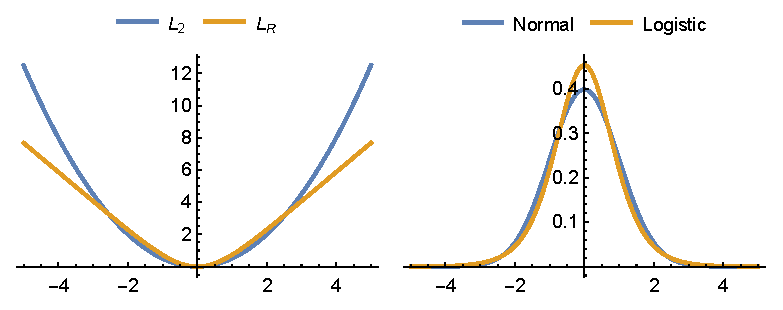
\includegraphics[width=1.05\columnwidth]{images/l2-lr-plot.eps}
    \caption{$L_2$ versus $L_R$ for typical values (left). Gaussian versus logistic probability density functions (right).}
    \label{fig:l2-lr-plot}
\end{figure}

\paragraph{Logistic performance model}
Now we assume the performance deviation $P_j-S_j$ has a logistic distribution with mean 0 and variance $\beta^2$. In general, the rating system administrator is free to set $\beta$ differently for each contest. Since shorter contests tend to be more variable, one reasonable choice might be to make $1/\beta^2$ proportional to the contest duration.

Given the mean and variance of the skill prior, the independent sum $P_j = S_j + (P_j-S_j)$ would have the same mean, and a variance that's increased by $\beta^2$. Unfortunately, we'll see that the logistic performance model implies a form of skill prior from which it's tough to extract a mean and variance. Even if we could, the sum does not yield a simple distribution.

For experienced players, we expect $S_j$ to contribute much less variance than $P_j-S_j$; thus, in our heuristic approximation, we take $P_j$ to have the same form of distribution as the latter. That is, we take $P_j$ to be logistic, centered at the prior rating $\mu^\pi_j = \argmax \pi_j$, with variance $\delta_j^2 = \sigma_j^2 + \beta^2$, where $\sigma_j$ will be given by \Cref{eq:variance}. This distribution is analytic and log-concave, so the same methods based on \Cref{thm:uniq-max} apply. 
Define the scale parameter $\bar\delta_j := \frac{\sqrt{3}}{\pi} \delta_j$. A logistic distribution with variance $\delta_j^2$ has cdf and pdf:
\begin{align*}
F_j(x) &= \frac { 1 } { 1 + e^{-(x-\mu^\pi_j)/\bar\delta_j} }
= \frac 12 \left(1 + \tanh\frac{x-\mu^\pi_j}{2\bar\delta_j} \right),
\\f_j(x) &= \frac { e^{(x-\mu^\pi_j)/\bar\delta_j} } { \bar\delta_j\left( 1 + e^{(x-\mu^\pi_j)/\bar\delta_j} \right)^2}
= \frac { 1 } { 4\bar\delta_j} \sech^2\frac{x-\mu^\pi_j}{2\bar\delta_j}.
\end{align*}

The logistic distribution satisfies two very convenient relations:
\begin{align*}
F'_j(x) = f_j(x) &= F_j(x) (1 - F_j(x)) / \bar\delta_j,
\\f'_j(x) &= f_j(x) (1 - 2F_j(x)) / \bar\delta_j,
\end{align*}
from which it follows that
\[d_j(p)
= \frac{1 - 2F_j(p)}{\bar\delta}
= \frac{-F_j(p)}{\bar\delta} + \frac{1 - F_j(p)}{\bar\delta}
= l_j(p) + v_j(p).\]

In other words, a tie counts as the sum of a win and a loss. This can be compared to the approach (used in Elo, Glicko, BAR, Topcoder, and Codeforces) of treating each tie as half a win plus half a loss.\footnote{Elo-MMR, too, can be modified to split ties into half win plus half loss. It's easy to check that \Cref{lem:decrease} still holds if $d_j(p)$ is replaced by
$w_l l_j(p) + w_v v_j(p)$,
provided that $w_l,w_v\in [0,1]$ and $|w_l-w_v|<1$.
In particular, we can set $w_l=w_v=0.5$. The results in \Cref{sec:properties} won't be altered by this change.}

Finally, putting everything together:
\[Q_i(p) = \sum_{j \succeq i} l_j(p) + \sum_{j \preceq i} v_j(p)
= \sum_{j \succeq i} \frac{-F_j(p)}{\bar\delta_j} + \sum_{j \preceq i} \frac{1 - F_j(p)}{\bar\delta_j}.\]
Our estimate for $P_i$ is the zero of this expression. The terms on the right correspond to probabilities of winning and losing against each player $j$, weighted by $1/\bar\delta_j$. Accordingly, we can interpret $\sum_{j\in \cP} (1-F_j(p))/\bar\delta_j$ as a weighted expected rank of a player whose performance is $p$. Similar to the performance computations in Codeforces and Topcoder, $P_i$ can thus be viewed as the performance level at which one's expected rank would equal $i$'s actual rank.


    \subsection{Belief update}
\label{sec:belief}

Having estimated $P_{i,t}$ in the first phase, the second phase is rather simple. Ignoring normalizing constants, \Cref{eq:new-obj} tells us that the pdf of the skill posterior can be obtained as the pointwise product of the pdfs of the skill prior and the performance model. When both factors are differentiable and log-concave, then so is their product. Its maximum is the new rating $\mu_{i,t}$; let's see how to compute it for the same two specializations of our model.

\paragraph{Gaussian performance model}
When the skill prior and performance model are Gaussian with known means and variances, multiplying their pdfs yields another known Gaussian. Hence, the posterior is compactly represented by its mean $\mu_{i,t}$, which coincides with the MAP and rating; and its variance $\sigma_{i,t}^2$, which is our \textbf{uncertainty} regarding the player's skill.

\paragraph{Logistic performance model}
When the performance model is non-Gaussian, the multiplication does not simplify so easily. By \Cref{eq:new-obj}, each round contributes an additional factor to the belief distribution. In general, we allow it to consist of a collection of simple log-concave factors, one for each round in which player $i$ has participated. Denote the participation history by
\[\cH_{i,t} := \{k\in\{1,\ldots,t\}:i\in\mathcal P_k\}.\]

Since each player can be considered in isolation, we'll omit the subscript $i$. Specializing to the logistic setting, each $k\in\cH_t$ contributes a logistic factor to the posterior, with mean $p_k$ and variance $\beta_k^2$. We still use a Gaussian initial prior, with mean and variance denoted by $p_0$ and $\beta_0^2$, respectively. Postponing the discussion of skill evolution to \Cref{sec:skill-drift}, for the moment we assume that $S_k=S_0$ for all $k$. The posterior pdf, up to normalization, is then
\begin{align}
&\pi_0(s) \prod_{k\in\cH_t} \Pr(P_k=p_k \mid S_k=s) \nonumber
\\&\propto \exp\left( -\frac{(s-p_0)^2}{2\beta_0^2} \right) \label{eq:posterior}
\prod_{k\in\cH_t} \sech^{2}\left( \frac\pi{\sqrt{12}} \frac{s-p_k} {\beta_k} \right).
\end{align}

Maximizing the posterior density amounts to minimizing its negative logarithm. Up to a constant offset, this is given by
\begin{align*}
L(s) &:= L_2\left(\frac{s-p_0}{\beta_0}\right)
+ \sum_{k\in\cH_t} L_R\left(\frac{s-p_k}{\beta_k}\right),
\\\text{where }L_2(x) &:= \frac 12 x^2\text{ and }
L_R(x) := 2\ln\left(\cosh \frac{\pi x}{\sqrt{12}}\right).
\end{align*}
\begin{equation}
\label{eq:loss}
\text{Thus, }L'(s) = \frac{s-p_0}{\beta_0^2} + \sum_{k\in\cH_t} \frac{\pi}{\beta_k\sqrt{3}} \tanh \frac{(s-p_k)\pi}{\beta_k\sqrt{12}}.
\end{equation}

$L'$ is continuous and strictly increasing in $s$, so its zero is unique: it is the MAP $\mu_t$. Similar to what we did in the first phase, we can solve for $\mu_t$ with binary search or other root-solving methods.

We pause to make an important observation. From \Cref{eq:loss}, the rating carries a rather intuitive interpretation: Gaussian factors in $L$ become $L_2$ penalty terms, whereas logistic factors take on a more interesting form as $L_R$ terms. From \Cref{fig:l2-lr-plot}, we see that the $L_R$ term behaves quadratically near the origin, but linearly at the extremities, effectively interpolating between $L_2$ and $L_1$ over a scale of magnitude $\beta_k$ 
%\aram{cite literature to justify this claim, and the next one? It would take more space to derive it ourselves}.

It is well-known that minimizing a sum of $L_2$ terms pushes the argument towards a weighted mean, while minimizing a sum of $L_1$ terms pushes the argument towards a weighted median. With $L_R$ terms, the net effect is that $\mu_t$ acts like a robust average of the historical performances $p_k$. Specifically, one can check that
\[\mu_t = \frac{\sum_k w_k p_k}{\sum_k w_k}, \text{ where } w_0 := \frac{1}{\beta_0^2} \text{ and }\]
\begin{equation}
\label{eq:average}
w_k := \frac{\pi}{(\mu_t-p_k)\beta_k\sqrt{3}}\tanh\frac{(\mu_t-p_k)\pi}{\beta_k\sqrt{12}} \text{ for }k\in\cH_t.
\end{equation}

$w_k$ is close to $1/\beta_k^2$ for typical performances, but can be up to $\pi^2/6$ times more as $|\mu_t-p_k| \rightarrow 0$, or vanish as $|\mu_t-p_k| \rightarrow\infty$. This feature is due to the thicker tails of the logistic distribution, as compared to the Gaussian, resulting in an algorithm that resists drastic rating changes in the presence of a few unusually good or bad performances. We'll formally state this \emph{robustness} property in \Cref{thm:robust}.

%Empirically, contest performances have indeed been seen to have thick tails, more like the logistic than the Gaussian (TODO citation).

\paragraph{Estimating skill uncertainty} While there is no easy way to compute the variance of a posterior in the form of \Cref{eq:posterior}, it will be useful to have some estimate $\sigma_t^2$ of uncertainty. There is a simple formula in the case where all factors are Gaussian. Since moment-matched logistic and normal distributions are relatively close (c.f. \Cref{fig:l2-lr-plot}), we apply the same formula:
\begin{equation}
\label{eq:variance}
\frac{1}{\sigma_t^2} := \sum_{k\in\{0\}\cup\cH_t}\frac{1}{\beta_k^2}.
\end{equation}
\section{Skill evolution over time}
\label{sec:skill-drift}
%This is an important component in applications, as players often train and improve between rounds.\footnote{This skill drift is modelled by almost all of the systems described in the introduction.} The time-varying skill is typically modelled by Gaussian noise, as we describe in \Cref{sec:skill-drift}.

Factors such as training and resting will change a player's skill over time. If we model skill as a static variable, our system will eventually grow so confident in its estimate that it will refuse to admit substantial changes. To remedy this, we introduce a skill evolution model, so that in general $S_t \neq S_{t'}$ for $t \neq t'$. Now rather than simply being equal to the previous round's posterior, the skill prior at round $t$ is given by
\begin{equation}
\label{eq:drift}
\pi_t(s) = \int \Pr(S_t = s \mid S_{t-1} = x) \Pr(S_{t-1} = x \mid P_{<t}) \,\dx.
\end{equation}

The factors in the integrand are the skill evolution model and the previous round's posterior, respectively. Following other Bayesian rating systems (e.g., Glicko, Glicko-2, and TrueSkill~\cite{G99, G12, HMG06}), we model the skill changes $S_t-S_{t-1}$ as independent zero-mean Gaussians. That is, $\Pr(S_t \mid S_{t-1}=x)$ is a Gaussian with mean $x$ and some variance $\gamma_t^2$. The Glicko system sets $\gamma_t^2$ proportionally to the time elapsed since the last update, corresponding to a continuous Brownian motion. Codeforces and Topcoder simply set $\gamma_t$ to a constant when a player participates, and zero otherwise, corresponding to changes that are in proportion to how often the player competes. Now we are ready to complete the two specializations of our rating system.

\paragraph{Gaussian performance model}
If both the prior and performance distributions at round $t-1$ are Gaussian, then the posterior is also Gaussian. Adding an independent Gaussian diffusion to our posterior on $S_{t-1}$ yields a Gaussian prior on $S_t$. By induction, the skill belief distribution forever remains Gaussian. This Gaussian specialization of the Elo-MMR framework lacks the R for robustness (see \Cref{thm:robust}), so we call it Elo-MM$\chi$.

\paragraph{Logistic performance model}
After a player's first contest round, the posterior in \Cref{eq:posterior} becomes non-Gaussian, rendering the integral in \Cref{eq:drift} intractable.

A very simple approach would be to replace the full posterior in \Cref{eq:posterior} by a Gaussian approximation with mean $\mu_t$ (equal to the posterior MAP) and variance $\sigma_t^2$ (given by \Cref{eq:variance}). As in the previous case, applying diffusions in the Gaussian setting is a simple matter of adding means and variances.

With this approximation, no memory is kept of the individual performances $P_t$. Priors are simply Gaussian, while posterior densities are the product of two factors: the Gaussian prior, and a logistic factor corresponding to the latest performance. To ensure robustness (see \Cref{sec:robust}), $\mu_t$ is computed as the argmax of this posterior \emph{before} replacement by its Gaussian approximation. We call the rating system that takes this approach Elo-MMR($\infty$).

As the name implies, it turns out to be a special case of Elo-MMR($\rho$). In the general setting with $\rho \in [0,\infty)$, we keep the full posterior from \Cref{eq:posterior}. Since we cannot tractably compute the effect of a Gaussian diffusion, we seek a heuristic derivation of the next round's prior, retaining a form similar to \Cref{eq:posterior} while satisfying many of the same properties as the intended diffusion.

\subsection{Desirable properties of a ``pseudodiffusion''}
\label{sec:desirable-props}
We begin by listing some properties that our skill evolution algorithm, henceforth called a ``pseudodiffusion'', should satisfy. The first two properties are natural:
\begin{itemize}[leftmargin=*]
\item \emph{Incentive-compatibility.} First and foremost, the pseudodiffusion must not break the incentive-compatibility of our rating system. That is, a rating-maximizing player should never be motivated to lose on purpose. (\Cref{thm:mono}).
\item \emph{Rating preservation.} The pseudodiffusion must not alter the $\argmax$ of the belief density. That is, the rating of a player should not change: $\mu^\pi_t = \mu_{t-1}$.
\end{itemize}
In addition, we borrow four properties of Gaussian diffusions:
\begin{itemize}[leftmargin=*]
\item \emph{Correct magnitude.} Pseudodiffusion with parameter $\gamma^2$ must increase the skill uncertainty, as measured by \Cref{eq:variance}, by $\gamma^2$.
\item \emph{Composability.} Two pseudodiffusions applied in sequence, first with parameter $\gamma_1^2$ and then with $\gamma_2^2$, must have the same effect as a single pseudodiffusion with parameter $\gamma_1^2 + \gamma_2^2$.
\item \emph{Zero diffusion.} In the limit as $\gamma \rightarrow 0$, the effect of pseudodiffusion must vanish, i.e., not alter the belief distribution.
\item \emph{Zero uncertainty.} In the limit as $\sigma_{t-1}\rightarrow 0$ (i.e., when the previous rating $\mu_{t-1}$ is a perfect estimate of $S_{t-1}$), our belief on $S_t$ must become Gaussian with mean $\mu_{t-1}$ and variance $\gamma^2$. Finer-grained information regarding the prior history $P_{\le t}$ must be erased.
\end{itemize}
In particular, Elo-MMR($\infty$) fails the \emph{zero diffusion} property because it simplifies the belief distribution, even when $\gamma=0$. In the proof of \Cref{thm:diffuse-prop}, we'll see that Elo-MMR($0$) fails the \emph{zero uncertainty} property. Thus, it is in fact necessary to have $\rho$ strictly positive and finite. In \Cref{sec:robust}, we'll come to interpret $\rho$ as a kind of inverse momentum.

\subsection{A heuristic pseudodiffusion algorithm}
\label{sec:pseudodiffusion}
Each factor in the posterior (see \Cref{eq:posterior}) has a parameter $\beta_k$. Define a factor's \textbf{weight} to be $w_k := 1/\beta_k^2$, which by \Cref{eq:variance} contributes to the \textbf{total weight} $\sum_k w_k=1/\sigma_t^2$. Here, unlike in \Cref{eq:average}, $w_k$ does not depend on $|\mu_t-p_k|$.

The approximation step of Elo-MMR($\infty$) replaces all the logistic factors by a single Gaussian whose variance is chosen to ensure that the total weight is preserved. In addition, its mean is chosen to preserve the player's rating, given by the unique zero of \Cref{eq:loss}. Finally, the diffusion step of Elo-MMR($\infty$) increases the Gaussian's variance, and hence the player's skill uncertainty, by $\gamma_t^2$; this corresponds to a decay in the weight.

To generalize the idea, we interleave the two steps in a continuous manner. The approximation step becomes a \textbf{transfer step}: rather than replace the logistic factors outright, we take away the same fraction from each of their weights, and \emph{place the sum of removed weights onto a new Gaussian factor}. In order for this operation to preserve ratings, the new factor must be centered at $\mu_{t-1}$. Since Gaussian pdfs compose, the prior Gaussian factor can be combined with the new one. The diffusion step becomes a \textbf{decay step}, reducing each factor's weight by the same fraction, chosen such that the overall uncertainty is increased by $\gamma_t^2$.

To make the idea precise, we generalize the posterior from \Cref{eq:posterior} with fractional \textbf{multiplicities} $\omega_k$; the $k$'th factor is raised to the power $\omega_k$. As a result, \Cref{eq:loss,eq:variance} become:
%initially set to $1$ for each $k\in\{0\}\cup\cH_t$. 
%The $k$'th factor is raised to the power $\omega_k$; in \Cref{eq:loss,eq:variance}, the corresponding term is multiplied by $\omega_k$.

\begin{align}
\label{eq:multiplicities}
L'(s) &= \frac{\omega_0(s-p_0)}{\beta_0^2} + \sum_{k\in\cH_t} \frac{\omega_k\pi}{\beta_k\sqrt{3}} \tanh \frac{(s-p_k)\pi}{\beta_k\sqrt{12}},\nonumber
\\\frac{1}{\sigma_t^2} &:= \sum_{k\in\{0\}\cup\cH_t}w_k,\quad\text{where }w_k := \frac{\omega_k}{\beta_k^2}.
\end{align}

For $\rho\in [0,\infty]$, the Elo-MMR($\rho$) algorithm continuously and simultaneously performs transfer and decay, with transfer proceeding at $\rho$ times the rate of decay. Holding $\beta_k$ fixed, changes to $\omega_k$ can be described in terms of changes to $w_k$:
\begin{align*}
\dot w_0 &= -r(t)w_0 + \rho r(t) \sum_{k\in\cH_t} w_k,
\\\dot w_k &= -(1+\rho)r(t)w_k \quad\text{for }k\in\cH_t,
\end{align*}
where the arbitrary decay rate $r(t)$ can be eliminated by a change of variable $\mathrm{d}\tau = r(t)\dt$. After some time $\Delta\tau$, the total weight will have decayed by a factor $\kappa := e^{-\Delta\tau}$, resulting in the new weights:
\begin{align*}
w_0^{new} &= \kappa w_0 + \left(\kappa-\kappa^{1+\rho}\right)\sum_{k\in\cH_t} w_k,
\\w_k^{new} &= \kappa^{1+\rho}w_k \quad\text{for }k\in\cH_t.
\end{align*}
In order for the uncertainty to increase from $\sigma_{t-1}^2$ to $\sigma_{t-1}^2+\gamma_t^2$, we must solve $\kappa/\sigma_{t-1}^2 = 1/(\sigma_{t-1}^2+\gamma_t^2)$ for the decay factor:
\[\kappa_t = \left(1 + \frac{\gamma_t^2}{\sigma_{t-1}^2}\right)^{-1}.\]

\setlength{\floatsep}{0pt}
\setlength{\textfloatsep}{1em}
\begin{algorithm}[t]
\caption{Elo-MMR($\rho,\beta, \gamma, \mu_{init}, \sigma_{init}$)}
\label{alg:main}
\begin{algorithmic}
\FORALL{rounds $t$}
\STATE $\mathcal P, \preceq, \succeq\; \gets$ outcome of round $t$
\FORALL{players $i\in\mathcal P$ in parallel}
\IF{$i$ has never competed before}
\STATE {$\mu_i, \sigma_i \gets \mu_{init}, \sigma_{init}$}
\STATE {$p_i, w_i \gets [\mu_i], [1/\sigma_i^2]$}
\ENDIF
%\STATE $\gamma \gets$ systemspecified()
\STATE diffuse($i$)
\STATE $\mu^\pi_i, \delta_i \gets \mu_i,\sqrt{\sigma_i^2 + \beta^2}$
%\STATE Make $\mu^\pi_i,\delta_i$ accessible to all threads in the next loop
\ENDFOR
%\STATE $E \gets$ getevidence()
\FORALL{players $i\in\mathcal P$ in parallel}
\STATE update($i$)
\ENDFOR
\ENDFOR
\end{algorithmic}
\end{algorithm}
\begin{algorithm}[t]
\caption{diffuse($i$)}
\label{alg:diffuse}
\begin{algorithmic}
\STATE $\kappa \gets (1+\gamma^2/\sigma_i^2)^{-1}$
\STATE $w_G, w_L \gets \kappa^\rho w_{i,0}, (1-\kappa^\rho) \sum_{k\geq 0} w_{i,k}$
\STATE $p_{i,0} \gets (w_G p_{i,0} + w_L \mu_i) / (w_G+w_L)$
\STATE $w_{i,0} \gets \kappa (w_G+w_L)$
\FORALL{$k > 0$}
\STATE $w_{i,k} \gets \kappa^{1+\rho}w_{i,k}$
\ENDFOR
\STATE $\sigma_i \gets \sigma_i / \sqrt\kappa$
\end{algorithmic}
\end{algorithm}
\begin{algorithm}[t]
\caption{update($i$)}
\label{alg:update}
\begin{algorithmic}
\STATE ${p \gets \mathop{\text{zero of}}\limits_{x \in \RR} \, \sum\limits_{j\preceq i}\frac{1}{\delta_j}\left( \tanh\frac {x - \mu^\pi_j} {2\bar\delta_j} - 1 \right) + \sum\limits_{j\succeq i}\frac{1}{\delta_j}\left( \tanh\frac {x - \mu^\pi_j} {2\bar\delta_j} + 1 \right)}$
\STATE $p_i$.push($p$)
\STATE $w_i$.push($1/\beta^2$)
\STATE $\mu_i \gets \mathop{\text{zero of}}\limits_{x \in \RR} \; w_{i,0}(x-p_{i,0}) + \sum\limits_{k>0} \frac{w_{i,k}\beta^2}{\bar\beta} \tanh \frac {x-p_{i,k}} {2\bar\beta}$
\end{algorithmic}
\end{algorithm}

\Cref{alg:main} details the full Elo-MMR($\rho$) rating system. Each round of competition yields a set of participants $\mathcal P$, along with their rank-ordering. New players are initialized with a Gaussian prior. Changes in player skill are modeled by \Cref{alg:diffuse}; note how the updated Gaussian term blends its old value with the new Gaussian term created by the transfer process. The first phase of \Cref{alg:update} estimates $P_t$ as the zero of a function of $x$. Finally, the second phase computes $\mu_t$ as the zero of another function. 

The hyperparameters $\rho,\beta,\gamma$ are domain-dependent, and can be set by standard hyperparameter search techniques. The system's invariance to translation and scale allows $\mu_{init},\sigma_{init}$ to be set arbitrarily; a common choice is $1500,350$~\cite{G12}. For convenience, we assume $\beta$ and $\gamma$ are fixed and use the shorthand $\bar\beta_k := \frac{\sqrt{3}}{\pi} \beta_k$. Whereas our exposition used global round indices, here a subscript $k$ corresponds to the $k$'th round in player $i$'s participation history.

\begin{theorem}
\label{thm:diffuse-prop}
\Cref{alg:diffuse} with $\rho\in(0,\infty)$ meets all of the properties listed in \Cref{sec:desirable-props}.
\end{theorem}

\begin{proof}
We go through each of the six properties in order.
\begin{itemize}[leftmargin=*]
    \item \emph{Incentive-compatibility.} This property will be stated in \Cref{thm:mono}. To ensure that its proof carries through, the relevant facts to note here are that the pseudodiffusion algorithm ignores the performances $p_k$, and centers the transferred Gaussian weight at the rating $\mu_{t-1}$, which is trivially monotonic in $\mu_{t-1}$.
    \item \emph{Rating preservation.} Recall that the rating is the unique zero of $L'$ in \Cref{eq:multiplicities}. To see that this zero is preserved, note that the decay and transfer operations multiply $L'$ by constants ($\kappa_t$ and $\kappa_t^\rho$, respectively), before adding the new Gaussian term, whose contribution to $L'$ is zero at its center.
    \item \emph{Correct magnitude.} Follows from our derivation for $\kappa_t$.
    \item \emph{Composability.} Follows from \emph{correct magnitude} and the fact that every pseudodiffusion follows the same differential equations.
    \item \emph{Zero diffusion.} As $\gamma\rightarrow 0$, $\kappa_t\rightarrow 1$. Provided that $\rho<\infty$, we also have $\kappa_t^\rho\rightarrow 1$. Hence, for all $k\in\{0\}\cup\cH_t$, $w_k^{new} \rightarrow w_k$.
    \item \emph{Zero uncertainty.} As $\sigma_{t-1}\rightarrow 0$, $\kappa_t\rightarrow 0$. The total weight decays from $1/\sigma_{t-1}^2$ to $\gamma^2$. Provided that $\rho > 0$, we also have $\kappa_t^\rho\rightarrow 0$, so these weights transfer in their entirety, leaving behind a Gaussian with mean $\mu_{t-1}$, variance $\gamma^2$, and no additional history. \qedhere
\end{itemize}
\end{proof}


\section{Theoretical Properties}
\label{sec:properties}
In this section, we see how the simplicity of the Elo-MMR formulas enables us to rigorously prove that the rating system is incentive-compatible, robust, and computationally efficient.

%\aram{erase this?} First, we discuss some properties that Elo-MMR has in common with the published systems of Codeforces and Topcoder, as well as the classical two-player systems Elo and Glicko. All of these systems propagate belief changes forward in time, never backward. This approach is simple, efficient, and has the benefit of never retroactively changing ratings from the past, nor the ratings of players who are not actively competing. In practice, Elo-MMR and Glicko also converge to the right results slightly faster than the others, by including an uncertainty parameter that starts high for new players.
\vspace{-.6em}
\subsection{Incentive-compatibility}
\label{sec:mono}

%\aram{erase this?} \emph{Aligned incentives} is one of our system's most important properties, so we devote this section to motivating, stating, and proving it. The main result, \Cref{thm:mono}, essentially guarantees that a player who seeks to improve their rating will never want to lose rounds, even if given the benefit of hindsight.

%To see that a "rational" rating system may fail monotonicity we begin with two examples.

%First, let's imagine a setting in which players typically maintain their "momentum"; that is, a player whose skill is improving rapidly, is expected to continue improving rapidly. A strategic player may then fake some momentum by intentionally performing at a weaker level, before returning to their actual level. The system may then believe that the player will continue to improve, granted inflated ratings until strong evidence arises to the contrary. This type of exploit was discovered in both the Topcoder rating system and the Pokemon Go rating system~\cite{forivsektheoretical, pokemongo}.%To show that this example is not just a hypothetical, \aram{cite Glicko-2, Topcoder, Pokemon Go}\cite{forivsektheoretical}.

%Next, we present a more subtle example. Consider a setting that presents players the choice between an easy challenge, which grants 1 point for partial success and 5 points for full success, or a hard challenge which grants 2 points for partial success and 10 points for full success.\footnote{This reward model is frequently used in coding competitions such as the International Olympiad of Informatics.} Experts with a high chance of a full success in the hard challenge should take it, whereas novices are likely to do better with the easy challenge. Let's suppose that, as a result, only experts attempt the hard challenges, and let's further suppose that a fraction of them fail to get a full success. Thus, there is a contingent of players with 2 points, all of whom are experts. If the rating system is powerful enough to know this, it may classify the 2-point players as stronger than the 5-point players, incentivizing a strategic novice to go for the lower point value!

%In summary, rating systems that are too powerful risk incentivizing players to perform cheap imitations of expert player behaviour, even when it undermines the game designer's objective for the player (e.g., to score more points). 

To demonstrate the need for incentive-compatibility, let's look at the consequences of violating this property in the Topcoder and Glicko-2 rating systems. These systems track a ``volatility'' for each player, which estimates the variance of their performances. A player whose recent performance history is more consistent would be assigned a lower volatility score, than one with wild swings in performance. The volatility acts as a multiplier on rating changes; thus, players with an extremely low or high performance will have their subsequent rating changes amplified.

While it may seem like a good idea to boost changes for players whose ratings are poor predictors of their performance, this feature has an exploit. By intentionally performing at a weaker level, a player can amplify future increases to an extent that more than compensates for the immediate hit to their rating. A player may even ``farm'' volatility by alternating between very strong and very weak performances. After acquiring a sufficiently high volatility score, the strategic player exerts their honest maximum performance over a series of contests. The amplification eventually results in a rating that exceeds what would have been obtained via honest play. This type of exploit was discovered in Glicko-2 as applied to the Pokemon Go video game~\cite{pokemongo}. Table 5.3 of ~\cite{forivsektheoretical} presents a milder violation in Topcoder competitions.

To get a realistic estimate of the severity of this exploit, we performed a simple experiment on the first five years of the Codeforces contest dataset (see \Cref{sec:datasets}). In \Cref{fig:topcoder-gaming}, we plot the rating evolution of the world's \#1 ranked competitive programmer, Gennady Korotkevich, better known as {\tt tourist}. In the \emph{control} setting, we plot his ratings according to the Topcoder and Elo-MMR($1$) systems. We contrast these against an \emph{adversarial} setting, in which we have {\tt tourist} employ the following strategy: for his first 45 contests, {\tt tourist} plays normally (exactly as in the unaltered data). For his next 45 contests, {\tt tourist} purposely falls to last place whenever his Topcoder rating is above 2975. Finally, {\tt tourist} returns to playing normally for an additional 15 contests.

This strategy mirrors the Glicko-2 exploit documented in~\cite{pokemongo}, and does not require unrealistic assumptions (e.g., we don't demand {\tt tourist} to exercise very precise control over his performances). Compared to a consistently honest {\tt tourist}, the volatility farming {\tt tourist} ended up \emph{523 rating points ahead} by the end of the experiment, with almost 1000 rating points gained in the last 15 contests alone. Transferring the same sequence of performances to the Elo-MMR($1$) system, we see that it not only is immune to such volatility-farming attacks, but it also penalizes the dishonest strategy with a rating loss that decays exponentially once honest play resumes.

\begin{figure}
\begin{minipage}{0.50\textwidth}
    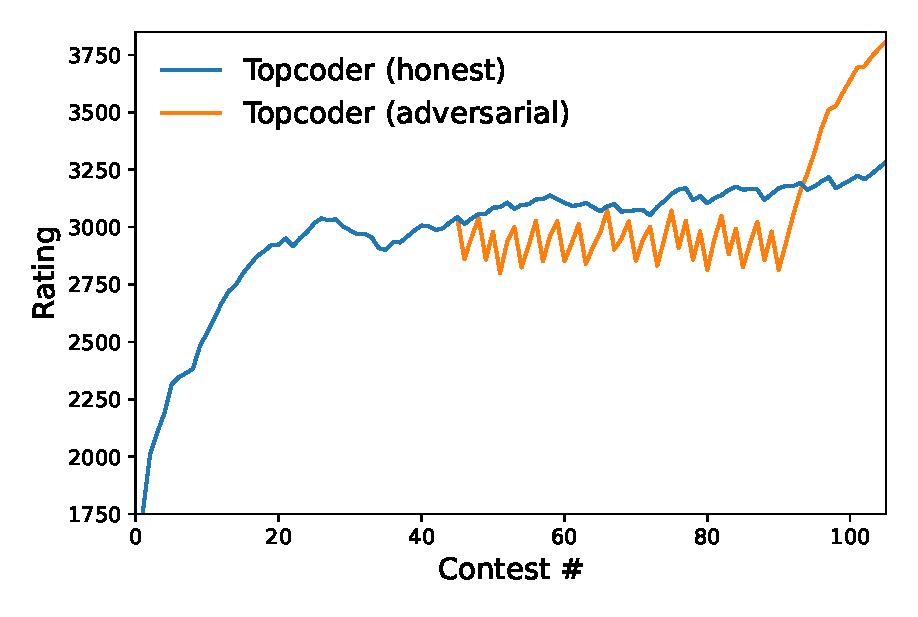
\includegraphics[width=0.95\textwidth]{images/topcoder.eps}
    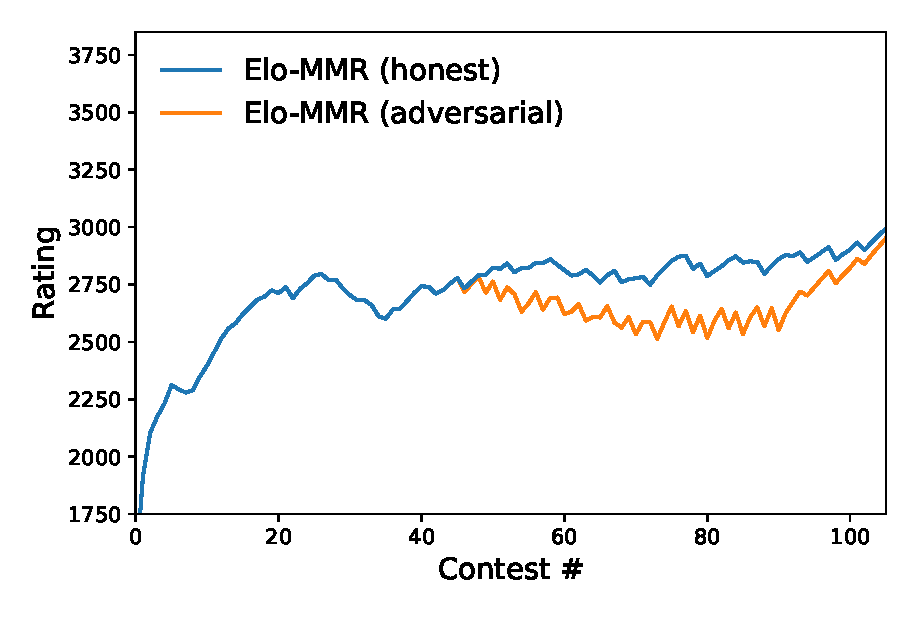
\includegraphics[width=0.95\textwidth]{images/elo-mmr.eps}
\end{minipage}
    \caption{Volatility farming attack on the Topcoder system.}
    \label{fig:topcoder-gaming}
\end{figure}

Recall that a key purpose of modeling volatility in Topcoder and Glicko-2 was to boost rating changes for inconsistent players. Remarkably, Elo-MMR achieves the same effect: we'll see in \Cref{sec:robust} that, for $\rho\in [0,\infty)$, Elo-MMR($\rho$) also boosts changes to inconsistent players. And yet, we'll now prove that no strategic incentive for purposely losing exists in \emph{any} version of Elo-MMR.

To this end, we need a few lemmas. Recall that, for the purposes of the algorithm, the performance $p_i$ is defined to be the unique zero of the function $Q_i(p) := \sum_{j \succ i} l_j(p) + \sum_{j \sim i} d_j(p) + \sum_{j \prec i} v_j(p)$, whose terms $l_j,d_j,v_j$ are contributed by opponents against whom $i$ lost, drew, or won, respectively. Wins (losses) are always positive (negative) contributions to a player's performance score:
\begin{lemma}
\label{lem:mono-term}
Adding a win term to $Q_i(\cdot)$, or replacing a tie term by a win term, always increases its zero. Conversely, adding a loss term, or replacing a tie term by a loss term, always decreases it.
\end{lemma}

\begin{proof}
By \Cref{lem:decrease}, $Q_i(p)$ is decreasing in $p$. Thus, adding a positive term will increase its zero whereas adding a negative term will decrease it. The desired conclusion follows by noting that, for all $j$ and $p$, $v_j(p)$ and $v_j(p)-d_j(p)$ are positive, whereas $l_j(p)$ and $l_j(p)-d_j(p)$ are negative.
\end{proof}

While not needed for our main result, a similar argument shows that performance scores are monotonic across the round standings:

\begin{theorem}
If $i \succ j$ (that is, player $i$ beats $j$) in a given round, then player $i$ and $j$'s performance estimates satisfy $p_i > p_j$.
\end{theorem}

\begin{proof}
If $i \succ j$ with $i,j$ adjacent in the rankings, then
\[Q_i(p) - Q_j(p) = \sum_{k\sim i}(d_k(p) - l_k(p)) + \sum_{k\sim j}(v_k(p) - d_k(p)) > 0.\]
for all $p$. Since $Q_i$ and $Q_j$ are decreasing functions, it follows that $p_i > p_j$. By induction, this result extends to the case where $i,j$ are not adjacent in the rankings.
\end{proof}

What matters for incentives is that performance scores be \emph{counterfactually} monotonic; meaning, if we were to alter the round standings, a strategic player will always prefer to place higher:
\begin{lemma}
\label{lem:mono-perf}
In any given round, holding fixed the relative ranking of all players other than $i$ (and holding fixed all preceding rounds), the performance $p_i$ is a monotonic function of player i's prior rating and of player $i$'s rank in this round.
\end{lemma}

\begin{proof}
Monotonicity in the prior rating follows directly from monotonicity of the self-tie term $d_i$ in $Q_i$. Since an upward shift in the rankings can only convert losses to ties to wins, monotonicity in contest rank follows from \Cref{lem:mono-term}. 
\end{proof}

Having established the relationship between round rankings and performance scores, the next step is to prove that, even with hindsight, players will always prefer their performance scores to be as high as possible:

\begin{lemma}
\label{lem:mono-rate}
Holding fixed the set of contest rounds in which a player has participated, their current rating is monotonic in each of their past performance scores.
\end{lemma}

\begin{proof}
The player's rating is given by the zero of $L'$ in \Cref{eq:multiplicities}. The pseudodiffusions of \Cref{sec:skill-drift} modify each of the $\beta_k$ in a manner that does not depend on any of the $p_k$, so they are fixed for our purposes. Hence, $L'$ is monotonically increasing in $s$ and decreasing in each of the $p_k$. Therefore, its zero is monotonically increasing in each of the $p_k$.

This is almost what we wanted to prove, except that $p_0$ is not a performance. Nonetheless, it is a function of the performances: specifically, a weighted average of historical ratings which, using this same lemma as an inductive hypothesis, are themselves monotonic in past performances. By induction, the proof is complete.
\end{proof}

Finally, we conclude that a rating-maximizing player is always motivated to improve their round rankings, or raw scores:

\begin{theorem}[Incentive-compatibility]
\label{thm:mono}
Holding fixed the set of contest rounds in which each player has participated, and the historical ratings and relative rankings of all players other than $i$, player $i$'s current rating is monotonic in each of their past rankings.
\end{theorem}

\begin{proof}
Choose any contest round in player $i$'s history, and consider improving player $i$'s rank in that round while holding everything else fixed. It suffices to show that player $i$'s current rating would necessarily increase as a result.

In the altered round, by \Cref{lem:mono-perf}, $p_i$ is increased; and by \Cref{lem:mono-rate}, player $i$'s post-round rating is increased. By \Cref{lem:mono-perf} again, this increases player $i$'s performance score in the following round. Proceeding inductively, we find that performance scores and ratings from this point onward are all increased.
\end{proof}

In the special cases of Elo-MM$\chi$ or Elo-MMR($\infty$), the rating system is ``memoryless'': the only data retained for each player are the current rating $\mu_{i,t}$ and uncertainty $\sigma_{i,t}$; detailed performance history is not saved. In this setting, we present a natural monotonicity theorem. A similar theorem was previously stated for the Codeforces system, albeit in an informal context without proof~\cite{Codeforces}.

\begin{theorem}[Memoryless Monotonicity]
In either the Elo-MM$\chi$ or Elo-MMR($\infty$) system, suppose $i$ and $j$ are two participants of round $t$. Suppose that the ratings and corresponding uncertainties satisfy $\mu_{i,t-1} \ge \mu_{j,t-1},\; \sigma_{i,t-1} = \sigma_{j,t-1}$. Then, $\sigma_{i,t} = \sigma_{j,t}$. Furthermore:

If $i \succ j$ in round $t$, then $\mu_{i,t} > \mu_{j,t}$.

If $j \succ i$ in round $t$, then $\mu_{j,t} - \mu_{j,t-1} > \mu_{i,t} - \mu_{i,t-1}$.
\end{theorem}

\begin{proof}
The new contest round will add a rating perturbation with variance $\gamma_t^2$, followed by a new performance with variance $\beta_t^2$. As a result,
\[\sigma_{i,t}
= \left( \frac{1}{\sigma_{i,t-1}^2 + \gamma_t^2} + \frac{1}{\beta_t^2} \right)^{-\frac 12}
= \left( \frac{1}{\sigma_{j,t-1}^2 + \gamma_t^2} + \frac{1}{\beta_t^2} \right)^{-\frac 12}
= \sigma_{j,t}.\]

The remaining conclusions are consequences of three properties: memorylessness, incentive-compatibility (\Cref{thm:mono}), and translation-invariance (ratings, skills, and performances are quantified on a common interval scale relative to one another).

Since the Elo-MM$\chi$ or Elo-MMR($\infty$) systems are memoryless, we may replace the initial prior and performance histories of players with any alternate histories of our choosing, as long as our choice is compatible with their current rating and uncertainty. For example, both $i$ and $j$ can be considered to have participated in the same set of rounds, with $i$ always performing at $\mu_{i,t-1}$. and $j$ always performing at $\mu_{j,t-1}$. Round $t$ is unchanged.

Suppose $i \succ j$. Since $i$'s historical performances are all equal or stronger than $j$'s, \Cref{thm:mono} implies $\mu_{i,t} > \mu_{j,t}$.

Suppose $j \succ i$. By translation-invariance, if we shift each of $j$'s performances, up to round $t$ and including the initial prior, upward by $\mu_{i,t-1} - \mu_{j,t-1}$, the rating changes between rounds will be unaffected. Players $i$ and $j$ now have identical histories, except that we still have $j\succ i$ at round $t$. Therefore, $\mu_{j,t-1} = \mu_{i,t-1}$ and, by \Cref{thm:mono}, $\mu_{j,t} > \mu_{i,t}$. Subtracting the equation from the inequality proves the second conclusion.
\end{proof}

\subsection{Robust response}
\label{sec:robust}

Another desirable property in many settings is robustness: a player's rating should not change too much in response to any one contest, no matter how extreme their performance. The Codeforces and TrueSkill systems lack this property, allowing for unbounded rating changes. Topcoder achieves robustness by clamping any changes that exceed a cap, which is initially high for new players but decreases with experience.

When $\rho>0$, Elo-MMR($\rho$) achieves robustness in a natural, smoother manner. To understand how, we look at the interplay between Gaussian and logistic factors in the posterior. Recall the notation in \Cref{eq:multiplicities}, describing the loss function and weights.

\begin{theorem}
\label{thm:robust}
In the Elo-MMR($\rho$) rating system, let
\[\Delta_+ := \lim_{p_t\rightarrow+\infty} \mu_{t}-\mu_{t-1},
\quad\Delta_- := \lim_{p_t\rightarrow-\infty}\mu_{t-1}-\mu_{t}.
\]
Then, for $\Delta_\pm \in \{\Delta_+, \Delta_-\}$,
\[\frac{\pi}{\beta_t\sqrt 3}
\left(w_0 + \frac{\pi^2}{6}\sum_{k\in\cH_{t-1}}w_k \right)^{-1}
\le \Delta_\pm
\le \frac{\pi}{\beta_t\sqrt 3}\frac{1}{w_0}.\]
%Then $\Delta_{min} \le \Delta < \Delta_{max}$, where
%\begin{align*}
%\Delta_{min} + \frac{2\pi\beta_t\beta_0^2}{\sqrt 3}(\sum_{k\in\mathcal R}\frac{1}{\beta_k})\tanh\frac{\Delta_{min}\pi}{4\sqrt 3 \beta_t} &= \frac{\pi\beta_0^2}{\beta_t\sqrt 3}
%\\\Delta_{max} &= \frac{\pi\beta_0^2}{\beta_t\sqrt 3}
%\end{align*}
\end{theorem}

\begin{proof}
The limits exist, by monotonicity. Using the fact that $0 < \frac{d}{dx}\tanh(x) \le 1$, differentiating $L'$ in \Cref{eq:multiplicities} yields
\[\forall s\in\mathbb R,\; w_0 \le L''(s)
\le w_0 + \frac{\pi^2}{6}\sum_{k\in\cH_{t-1}}w_k.\]

Now, the performance at round $t$ adds a new term with multiplicity one to $L'(s)$: its value is
$\frac{\pi}{\beta_k\sqrt{3}} \tanh \frac{(s-p_k)\pi}{\beta_k\sqrt{12}}$.

As a result, for every $s\in\mathbb R$, in the limit as $p_t\rightarrow\pm\infty$, $L'(s)$ increases by $\mp\frac{\pi}{\beta_t\sqrt 3}$. Since $\mu_{t-1}$ was a zero of $L'$ without this new term, we now have
$L'(\mu_{t-1}) \rightarrow \mp\frac{\pi}{\beta_t\sqrt 3}.$ Dividing by the former inequalities yields the desired result.
\end{proof}

The proof reveals that the magnitude of $\Delta_{\pm}$ depends inversely on that of $L''$ in the vicinity of the current rating, which in turn is related to the derivative of the $\tanh$ terms. If a player's performances vary wildly, the tanh terms will be widely dispersed, so any potential rating value will necessarily be in the tail ends of most of the terms. Tails contribute very small derivatives, enabling a larger rating change. Conversely, the $\tanh$ terms of a player with a very consistent performance history will contribute large derivatives, so the bound on their rating change will be small.

Thus, Elo-MMR naturally caps the rating changes of all players, and the cap is smaller for consistent performers. The cap will increase after an extreme performance, providing a similar ``momentum'' to the Topcoder and Glicko-2 systems, but without sacrificing incentive-compatibility (\Cref{thm:mono}).

We can compare the lower and upper bound in \Cref{thm:robust}: their ratio is on the same order as the fraction of the total weight that is held by the normal term. Recall that $\rho$ is the weight transfer rate: larger $\rho$ results in more weight being transferred into $w_0$; in this case, the lower and upper bound tend to stay close together. Conversely, the momentum effect is more pronounced when $\rho$ is small. In the extreme case $\rho=0$, $w_0$ vanishes for experienced players, so a sufficiently volatile player would be subject to correspondingly large rating updates. In the extended version of this paper, we quantify an asymptotic steady state for the weights, and argue that $1/\rho$ can be thought of as a momentum parameter.

\subsection{Runtime analysis and optimizations}
\label{sec:runtime}
Let's look at the computation time needed to process a round with participant set $\mathcal P$, where we again omit the round subscript. Each player $i$ has a participation history $\cH_i$.

Estimating $P_i$ entails finding the zero of a monotonic function with $O(|\mathcal P|)$ terms, and then obtaining the rating $\mu_i$ entails finding the zero of another monotonic function with $O(|\cH_i|)$ terms. Using either of the Illinois or Newton methods, solving these equations to precision $\epsilon$ takes $O(\log\log\frac 1\epsilon)$ iterations. As a result, the total runtime needed to process one round of competition is
\[O\left(\sum_{i\in\mathcal P}(|\mathcal P| + |\cH_i|) \log\log\frac 1\epsilon\right).\]
This complexity is more than adequate for Codeforces-style competitions with thousands of contestants and history lengths up to a few hundred. Indeed, we were able to process the entire history of Codeforces on a small laptop in less than half an hour. Nonetheless, it may be cost-prohibitive in truly massive settings, where $|\mathcal P|$ or $|\cH_i|$ number in the millions. Fortunately, it turns out that both functions may be compressed down to a bounded number of terms, with negligible loss of precision.

\paragraph{Adaptive subsampling}
In \Cref{sec:bayes_model}, we used Doob's consistency theorem to argue that our estimate for $P_i$ is consistent. Specifically, we saw that $O(1/\epsilon^2)$ opponents are needed to get the typical error below $\epsilon$. Thus, we can subsample the set of opponents to include in the estimation, omitting the rest. Random sampling is one approach. A more efficient approach chooses a fixed number of opponents whose ratings are closest to that of player $i$, as these are more likely to provide informative match-ups. On the other hand, if the setting requires incentive-compatibility to hold exactly, then one must avoid choosing different opponents for each player.

\paragraph{History compression}
Similarly, it's possible to bound the number of stored factors in the posterior. Our skill-evolution algorithm decays the weights of old performances at an exponential rate. Thus, the contributions of all but the most recent $O(\log\frac 1\epsilon)$ terms are negligible. Rather than erase the older logistic terms outright, we recommend replacing them with moment-matched Gaussian terms, similar to the transfers in \Cref{sec:skill-drift} with $\kappa_t=0$. Since Gaussians compose easily, a single term can then summarize an arbitrarily long prefix of the history.

Substituting $1/\epsilon^2$ and $\log\frac 1\epsilon$ for $|\cP|$ and $|\cH_i|$, respectively, the runtime of Elo-MMR with both optimizations becomes
\[O\left(\frac {|\mathcal P|}{\epsilon^2} \log\log\frac 1\epsilon\right).\]

If the contests are \emph{extremely large}, so that $\Omega(1/\epsilon^2)$ opponents have a rating and uncertainty in the same $\epsilon$-width bucket as player $i$, then it's possible to do even better: up to the allowed precision $\epsilon$, the corresponding terms can be treated as duplicates. Hence, their sum can be determined by counting how many of these opponents win, lose, or tie against player $i$. Given the pre-sorted list of ranks of players in the bucket, two binary searches would yield the answer. In practice, a single bucket might not contain enough participants, so we sample enough buckets to yield the desired precision.

\paragraph{Simple parallelism}
Since each player's rating computation is independent, the algorithm is embarrassingly parallel. Threads can read the same global data structures, so each additional thread contributes only $O(1)$ memory overhead.

% \subsection{erase all this, or present in a different way?}

% Imagine a player who performs very consistently over a long period of time, repeatedly achieving $p_i = 1000$ until convergence. Now, perhaps as a result of attending an intensive training camp in Petrozavodsk, their skill changes dramatically. From this point on, they consistently achieve $p_i = 3000$.

% How does each rating system respond to the first such surprise occurrence? Elo-MMR treats the new result as a fluke, an outlier that ought to be ignored. The player gains 48 points; as a result of the parameters we set, this is the maximum possible for an experienced player as $p_i \rightarrow \infty$. In practice, ratings may change by more than 48, as the maximum depends on existing fluctuations in their history; here we're looking at the extreme example of a player with a history of always performing at exactly $p_i = 1000$.

% \begin{figure}
%     \centering
%     \includegraphics[width=\columnwidth]{images/ResponsePlot.png}
%     \caption{An accelerated convergence effect in the presence of sustained improved performances.}
%     \label{fig:accelerated}
% \end{figure}

% Had we tried to perform outlier reduction in a memoryless fashion, we would continue to increase the rating by 48 per match, oblivious to the possibility that the player truly did experience a sudden improvement. In Elo-MMR, the outlier status of a performance is treated as tentative. If later matches support the hypothesis of having improved, the rating will increase by an additional 63 points, followed by over 100 points in each of the third and following matches, as plotted by the blue curve above.

% After six consecutive matches with $p_i = 3000$, the rating is 1875 and very unstable (even though $\sigma_i$ is unchanged!). The system is no longer sure which to trust: the extensive history at level 1000, or the smaller number of recent matches at level 3000. Depending on what comes next, the player's rating can very quickly fall toward 1000 or rise toward 3000. However, note that in either case, the change will not overshoot, say to 5000, unless enough new evidence is accumulated at that level. As the $p_i=3000$ streak continues, the seventh match on the blue curve jumps by a whopping 566 points. As the player's rating converges to 3000, the old $p_i = 1000$ data acquires outlier status, thus speeding convergence.

% In contrast, while a system such as Codeforces does not compute $p_i$ values in quite in the same way, we can obtain a good approximation by removing outlier reduction from Elo-MMR, effectively treating the performances to be averaged as normal instead of logistic measurements. This makes the system effectively memoryless, since it turns out that each match simply moves the rating about 16\% closer to the new $p_i$ value, independent of the history. With this change, we obtain the orange curve, which jumps a whopping 320 points at the very first performance. Indeed, there is no limit: if you could find players whose ratings are extremely high, and beat them even once, your rating would take arbitrarily large leaps.

% Note that this is not quite true of Topcoder, which incorporates a hack that caps the maximum rating change: if Topcoder's update formula demands too large a change, the cap kicks in. In contrast, Elo-MMR's cap is a natural and smooth consequence of its update formula and is sensitive to whether a change is charting new territory, or merely confirming a plausible hypothesis. Topcoder does attempt to make the magnitude of its updates sensitive to the amount of fluctuation in a player's history, using a volatility measure, but this measure does not account for the direction of the changes, resulting in the non-monotonicity flaw mentioned above.

% Notwithstanding arguments that a high rating ought to properly be earned over multiple matches rather than a single fluke, the other danger is that these observations also hold in reverse: one bad day on Codeforces can seriously damage one's rating and negate several rounds of steady progress. By using heavy-tailed logistic distributions everywhere, Elo-MMR understands that unusually high or low performances do occasionally occur, and one round in isolation is never a reliable signal.

% Interestingly, despite the slow start, the blue curve ultimately converges faster than the orange one. Since Elo-MMR uses its memory to dynamically adapt its view of potential outliers, it overtakes the orange curve as soon as new evidence outweighs the old hypothesis!

% \subsection{Inflation and division boundary artifacts: erase or rewrite?}

% The code and ratings of real Codeforces members as computed by Elo-MMR are available at https://github.com/EbTech/EloR. Original Codeforces ratings are at http://codeforces.com/ratings. One striking difference is massive inflation in the Codeforces system. Gennady Korotkevich, best known by his competitive programming handle ``tourist'', has been the reigning world champion for years. Toward the end of 2011, his rating reached a new ceiling of about 2700 according to both systems. However, as of this writing, his rating on Elo-MMR has increased by about 300 additional points, while on Codeforces it increased by almost 900. To get a sense of the magnitude of this change, 900 points is the difference between an average member and a Grandmaster! Indeed, most of the variance in the Codeforces system is concentrated at the top, with much smaller rating differences between beginner and intermediate members. This is caused by certain ad hoc elements of the system that are not founded on any rigorous model.
\section{Experiments}
\label{sec:experiments}
In this section, we compare various rating systems on real-world datasets, mined from several sources that will be described in \Cref{sec:datasets}. The metrics are runtime and predictive accuracy, as described in \Cref{sec:metrics}. Implementations of all rating systems, dataset mining, and additional processing used in our experiments can be found at {\tt\url{https://github.com/EbTech/Elo-MMR}}.

We compare Elo-MM$\chi$ and Elo-MMR($\rho$) against the industry-tested rating systems of Codeforces and Topcoder. For a fairer comparison, we hand-coded efficient versions of all four algorithms in the safe subset of Rust, parellelized using the Rayon crate; as such, the Rust compiler verifies that they contain no data races~\cite{stone2017rayon}. Our implementation of Elo-MMR($\rho$) makes use of the optimizations in \Cref{sec:runtime}, bounding both the number of sampled opponents and the history length by 500. In addition, we test the improved TrueSkill algorithm of \cite{NS10}, basing our code on an open-source implementation of the same algorithm. The inherent seqentiality of its message-passing procedure prevented us from parallelizing it. All experiments were run on a 2.0 GHz 24-core Skylake machine with 24 GB of memory.

\paragraph{Hyperparameter search}
To ensure fair comparisons, we ran a separate grid search for each triple of algorithm, dataset, and metric, over all of the algorithm's hyperparameters. The hyperparameter set that performed best on the first 10\% of the dataset, was then used to test the algorithm on the remaining 90\% of the dataset. 

%We find that our rating performs slightly better than all competitors in terms of predictive power. In terms of computational time however, we show that Elo-MMR is up to an order of magnitude faster than Codeforces.

\subsection{Datasets}
\label{sec:datasets}

\begin{table}[t]
\begin{tabular}{l|l|l}
\hline
\textbf{Dataset} & \textbf{\# contests} & \textbf{avg. \# participants / contest} \\ \hline
Codeforces       & 1087                & 2999                                     \\ %\hline
Topcoder         & 2023                & 403                                   \\ %\hline
Reddit           & 1000                & 20                                       \\
%\hline
Synthetic        & 50                  & 2500     \\ \hline
\end{tabular}
    \caption{Summary of test datasets.}
    \label{tab:dataset-summary}
    \vspace{-1.2em}
\end{table}

Due to the scarcity of public domain datasets for rating systems, we mined three datasets to analyze the effectiveness of our system. The datasets were mined using data from each source website's inception up to October 9th, 2020. We also created a synthetic dataset to test our system's performance when the data generating process matches our theoretical model. Summary statistics of the datasets are presented in \Cref{tab:dataset-summary}.

\paragraph{Codeforces contest history}
This dataset contains the current entire history of rated contests ever run on codeforces.com, the dominant platform for online programming competitions. The Codeforces platform has over 850K users, over 300K of whom are rated, and has hosted over 1000 contests to date. Each contest has a couple thousand participants on average. A typical contest takes 2 to 3 hours and contains 5 to 8 problems. Players are ranked by total points, with more points typically awarded for tougher problems and for early solves. They may also attempt to ``hack'' one another's submissions for bonus points, identifying test cases that break their solutions. %The sheer number of highly motivated participants in these competitions, as well as their very accessible data API, made it the top choice for our explorations.
\looseness=-1

\paragraph{Topcoder contest history}
This dataset contains the current entire history of algorithm contests ever run on the topcoder.com. Topcoder is a predecessor to Codeforces, with over 1.4 million total users and a long history as a pioneering platform for programming contests. It hosts a variety of contest types, including over 2000 algorithm contests to date. The scoring system is similar to Codeforces, but its rounds are shorter: typically 75 minutes with 3 problems.

\paragraph{SubredditSimulator threads}
This dataset contains data scraped from the current top-1000 most upvoted threads on the website {\tt\url{reddit.com/r/SubredditSimulator/}}. Reddit is a social news aggregation website with over 300 million users. The site itself is broken down into sub-sites called subreddits. Users then post and comment to the subreddits, where the posts and comments receive votes from other users. In the subreddit SubredditSimulator, users are language generation bots trained on text from other subreddits. Automated posts are made by these bots to SubredditSimulator every 3 minutes, and real users of Reddit vote on the best bot. Each post (and its associated comments) can thus be interpreted as a round of competition between the bots who commented. 

\paragraph{Synthetic data}
This dataset contains 10K players, with skills and performances generated according to the Gaussian generative model in \Cref{sec:bayes_model}. Players' initial skills are drawn i.i.d. with mean $1500$ and variance $350^2$. Players compete in all rounds, and are ranked according to independent performances with variance $200^2$. Between rounds, we add i.i.d. Gaussian increments with variance $35^2$ to each of their skills.
% Uh is this the logistic or the Gaussian model??????

\subsection{Evaluation metrics}
\label{sec:metrics}
To compare the different algorithms, we define two measures of predictive accuracy. Each metric will be defined on individual contestants in each round, and then averaged:
\[\mathrm{\bf aggregate(metric)} := \frac{\sum_t \sum_{i\in\mathcal P_t} \mathrm{\bf metric}(i,t)}{\sum_t |\mathcal P_t|}.\]

\paragraph{Pair inversion metric~\cite{HMG06}}
Our first metric computes the fraction of opponents against whom our ratings predict the correct pairwise result, defined as the higher-rated player either winning or tying: 
\[\mathrm{\bf pair\_inversion}(i,t) := \frac{\text{\# correctly predicted matchups}}{|\mathcal P_t|-1} \times 100\%.\]
This metric was used in the original evaluation of TrueSkill~\cite{HMG06}.

\paragraph{Rank deviation}
Our second metric compares the rankings with the total ordering that would be obtained by sorting players according to their prior rating. The penalty is proportional to how much these ranks differ for player $i$:
\[\mathrm{\bf rank\_deviation}(i,t) := \frac{|\text{actual rank} - \text{predicted rank}|}{|\mathcal P_t|-1} \times 100\%.\]
In the event of ties, among the ranks within the tied range, we use the one that comes closest to the rating-based prediction.

% \paragraph{Entropy-based metric}
% For this metric, we evaluate the interpretability of the system ratings. As specified in \Cref{sec:bayes_model}, we assume player performances follow a Bradley-Terry model\paul{add BT and thurstone to this section}. In particular, we assume the probability of participants $i$ beating $j$ in a round $R$ is predicted by the simple formula \[\Pr[i \succ j] = \frac{1}{1 + 10^{\frac{\mu_i - \mu_j}{400}}}.\]
% As previously stated, this formula is assumed by the classic Elo rating system as well as the Codeforces rating system~\cite{...}, with the main benefit being that players can easily interpret the meaning of their ratings. To measure the interpretability, we measure the distance between the win distribution implied by the rating system and the actual win distribution. One way to do this is to measure the cross-entropy (which is equal to the KL-divergence up to an additive constant) via the follow formula:
% \[\mathrm{entropy} = -\frac{1}{\text{\# total pairs}} \sum_{\substack{i,j \in R \\ i \succ j}} \log \frac{1}{1 + 10^{\frac{\mu_i - \mu_j}{400}}}.\]

\subsection{Empirical results}
\begin{table*}
\begin{tabular}{l|ll|ll|ll|ll|ll}
 \hline
\multirow{2}{*}{\textbf{Dataset}} &
  \multicolumn{2}{l|}{\textbf{Codeforces}} &
  \multicolumn{2}{l|}{\textbf{Topcoder}} &
  \multicolumn{2}{l|}{\textbf{TrueSkill}} &
  \multicolumn{2}{l|}{\textbf{Elo-MM$\boldsymbol\chi$}} & 
  \multicolumn{2}{l}{\textbf{Elo-MMR($\boldsymbol\rho$)}} \\ \cline{2-11}
&
  pair inv. &
  rank dev. &
  pair inv. &
  rank dev. &
  pair inv. &
  rank dev. &
  pair inv. &
  rank dev. &
  pair inv. &
  rank dev. \\ \hline
Codeforces & 78.3\% & 14.9\% & 78.5\% & 15.1\% & 61.7\% & 25.4\% & 78.5\% & 14.8\% & {\bf 78.6}\% & {\bf 14.7}\% \\ %\hline
Topcoder  & 72.6\%     & 18.5\%     & 72.3\% & 18.7\%  & 68.7\% & 20.9\% & 73.0\% & 18.3\% & {\bf 73.1}\% & {\bf 18.2}\% \\ %\hline
Reddit     & 61.5\%     & 27.3\%     & 61.4\% & 27.4\% & 61.5\% & {\bf 27.2}\% & 61.6\% & 27.3\% & {\bf 61.6\%} & 27.3\% \\ %\hline
Synthetic  & {\bf 81.7\%}     & 12.9\%     & {\bf 81.7}\% & {\bf 12.8}\% & 81.3\% & 13.1\% & {\bf 81.7}\% & {\bf 12.8}\% & {\bf 81.7\%} & {\bf 12.8\%} \\ \hline
\end{tabular}
\caption{Performance of each rating system on the pairwise inversion and rank deviation metrics. Bolded entries denote the best performances (highest pair inv. or lowest rank dev.) on each metric and dataset.}
\label{tbl:metric-results}
\vspace{-1.2em}
\end{table*}

\begin{table}
\begin{tabular}{l|lllll}
\hline
\textbf{Dataset} & \textbf{CF} & \textbf{TC} & \textbf{TS} & \textbf{Elo-MM$\boldsymbol\chi$} & \textbf{Elo-MMR($\boldsymbol\rho$)} \\ \hline
Codeforces & 212.9 & 72.5 & 67.2 & {\bf 31.4} & 35.4\\
Topcoder   & 9.60 & {\bf 4.25} & 16.8 & 7.00 & 7.52\\
Reddit     & 1.19  & 1.14 & {\bf 0.44} & 1.14 & 1.42 \\
Synthetic  & 3.26  & 1.00 & 2.93 & {\bf 0.81} & 0.85 \\ \hline
\end{tabular}
\caption{Total compute time over entire dataset, in seconds.}
\label{tbl:time-results}
\vspace{-1.2em}
\end{table}

Recall that Elo-MM$\chi$ has a Gaussian performance model, matching the modeling assumptions of Topcoder and TrueSkill. Elo-MMR($\rho$), on the other hand, has a logistic performance model, matching the modeling assumptions of Codeforces and Glicko. While $\rho$ was included in the hyperparameter search, in practice we found that all values between $0$ and $1$ produce very similar results.

To ensure that errors due to the unknown skills of new players don't dominate our metrics, we excluded players who had competed in less than 5 total contests. In most of the datasets, this reduced the performance of our method relative to the others, as our method seems to converge more accurately. Despite this, we see in \Cref{tbl:metric-results} that both versions of Elo-MMR outperform the other rating systems in both the pairwise inversion metric and the ranking deviation metric.
\looseness=-1

We highlight a few key observations. First, significant performance gains are observed on the Codeforces and Topcoder datasets, despite these platforms' rating systems having been designed specifically for their needs. Our gains are smallest on the synthetic dataset, for which all algorithms perform similarly. This might be in part due to the close correspondence between the generative process and the assumptions of these rating systems. Furthermore, the synthetic players compete in all rounds, enabling the system to converge to near-optimal ratings for every player. Finally, the improved TrueSkill performed well below our expectations, despite our best efforts to improve it. We suspect that the message-passing numerics break down in contests with a large number of individual participants. The difficulties persisted in all TrueSkill implementations that we tried, including on Microsoft's popular {\tt Infer.NET} framework~\cite{InferNET18}. To our knowledge, we are the first to present experiments with TrueSkill on contests where the number of participants is in the hundreds or thousands. In preliminary experiments, TrueSkill and Elo-MMR score about equally when the number of ranks is less than about 60.

Now, we turn our attention to \Cref{tbl:time-results}, which showcases the computational efficiency of Elo-MMR. On smaller datasets, it performs comparably to the Codeforces and Topcoder algorithms. However, the latter suffer from a quadratic time dependency on the number of contestants; as a result, Elo-MMR outperforms them by almost an order of magnitude on the larger Codeforces dataset.

Finally, in comparisons between the two Elo-MMR variants, we note that while Elo-MMR($\rho$) is more accurate, Elo-MM$\chi$ is always faster. This has to do with the skill drift modeling described in \Cref{sec:skill-drift}, as every update in Elo-MMR($\rho$) must process $O(\log\frac 1\epsilon)$ terms of a player's competition history.

\section{Conclusions}
This paper introduces the Elo-MMR rating system, which is in part a generalization of the two-player Glicko system, allowing any number of players. By developing a Bayesian model and taking the limit as the number of participants goes to infinity, we obtained simple, human-interpretable rating update formulas. Furthermore, we saw that the algorithm is incentive-compatible, robust to extreme performances, asymptotically fast, and embarrassingly parallel. To our knowledge, our system is the first to rigorously prove all these properties in a setting with more than two individually ranked players. In terms of practical performance, we saw that it outperforms existing industry systems in both prediction accuracy and computation speed.
%In particular, we compare against the popular CodeForces, Topcoder, and TrueSkill rating systems, which are deployed on platforms with hundreds of thousands to millions of users.

This work can be extended in several directions. First, the choices we made in modeling ties, pseudodiffusions, and opponent subsampling are by no means the only possibilities consistent with our Bayesian model of skills and performances. Second, it may be possible to further improve accuracy by fitting more flexible performance and skill evolution models to application-specific data.

Another useful extension would be to team competitions. Given a performance model for teams, Elo-MMR infers each team's performance. To make this useful in settings where teams are frequently reassigned, we must model teams in terms of their individual members; unfortunately, it's not possible to precisely infer an individual's performance from team rankings alone. Therefore, it becomes necessary to condition an individual's skill on their team's performance. In the case where a team's performance is modeled as the sum of its members' independent Gaussian contributions, elementary facts about multivariate Gaussian distributions enable posterior skill inferences at the individual level. Generalizing this approach to other models remains an open challenge.

% Probably redundant: The algorithm itself is trivially parallelizable, and further speedup can be attained through a simple sub-sampling strategy. We believe there is potential to improve the performance even more, either through a more sophisticated sub-sampling strategy, interpolation, or by combining our two-phase approach with a factor graph framework similar to that of TrueSkill~\cite{HMG06, KFL01}. 

Over the past decade, online competition communities such as Codeforces have grown exponentially. As such, considerable work has gone into engineering scalable and reliable rating systems. Unfortunately, many of these systems have not been rigorously analyzed in the academic community. We hope that our paper and open-source release will open new explorations in this area.

%In addition, we invite non-technical sporting communities, such as the Spartan Race and DanceSport, to find uses of our skill estimation package.

% IMPORTANT: This conference is double blind, which (aside from anonymous authors) means that we cannot post links to our git or have acknowledgements.

\section*{Acknowledgements}
The authors are indebted to Daniel Sleator and Danica J. Sutherland for initial discussions that helped inspire this work, and to Nikita Gaevoy for the open-source improved TrueSkill upon which our implementation is based. Experiments in this paper are funded by a Google Cloud Research Grant. The second author is supported by a VMWare Fellowship and the Natural Sciences and Engineering Research Council of Canada.

\balance

%\appendix
%\section*{Appendix}
\begingroup
\def\thetheorem{\ref{lem:decrease}}
\begin{lemma}
If $f_i$ is continuously differentiable and log-concave, then the functions $l_i,d_i,v_i$ are continuous, strictly decreasing, and
\[l_i(p) < d_i(p) < v_i(p) \text{ for all }p.\]
\end{lemma}
\addtocounter{theorem}{-1}
\endgroup
\begin{proof}
Continuity of $F_i,f_i,f'_i$ implies that of $l_i,d_i,v_i$. It's known~\cite{concave} that log-concavity of $f_i$ implies log-concavity of both $F_i$ and $1-F_i$. As a result, $l_i$, $d_i$, and $v_i$ are derivatives of strictly concave functions; therefore, they are strictly decreasing. In particular, each of

\[v'_i(p) = \frac{f'_i(p)}{F_i(p)} - \frac{f_i(p)^2}{F_i(p)^2},\quad
l'_i(p) = \frac{-f'_i(p)}{1-F_i(p)} - \frac{f_i(p)^2}{(1-F_i(p))^2},\]

are negative for all $p$, so we conclude that

\begin{align*}
d_i(p) - v_i(p)
= \frac{f'_i(p)}{f_i(p)} - \frac{f_i(p)}{F_i(p)}
&= \frac{F_i(p)}{f_i(p)} v'_i(p)
< 0,
\\l_i(p) - d_i(p)
= -\frac{f'_i(p)}{f_i(p)} -\frac{f_i(p)}{1-F_i(p)}
&= \frac{1-F_i(p)}{f_i(p)} l'_i(p)
< 0.
\end{align*}

\end{proof}

\begingroup
\def\thetheorem{\ref{thm:uniq-max}}
\begin{theorem}
Suppose that for all $j$, $f_j$ is continuously differentiable and log-concave. Then the unique maximizer of $\Pr(P_i=p\mid E^L_i,E^W_i)$ is given by the unique zero of
\[Q_i(p) = \sum_{j \succ i} l_j(p) + \sum_{j \sim i} d_j(p) + \sum_{j \prec i} v_j(p).\]
\end{theorem}
\addtocounter{theorem}{-1}
\endgroup

\begin{proof}
First, we rank the players by their buckets according to $\floor{P_j/\epsilon}$, and take the limiting probabilities as $\epsilon\rightarrow 0$:
\begin{align*}
    \Pr(\floor{\frac{P_j}\epsilon} > \floor{\frac{p}\epsilon})
    &= \Pr(p_j \ge \epsilon\floor{\frac{p}\epsilon} + \epsilon)
    \\&= 1 - F_j(\epsilon\floor{\frac{p}\epsilon} + \epsilon)
    \rightarrow 1 - F_j(p),
    \\\Pr(\floor{\frac{P_j}\epsilon} < \floor{\frac{p}\epsilon})
    &= \Pr(p_j < \epsilon\floor{\frac{p}\epsilon})
    \\&= F_j(\epsilon\floor{\frac{p}\epsilon})
    \rightarrow F_j(p),
    \\\frac 1\epsilon \Pr(\floor{\frac{P_j}\epsilon} = \floor{\frac{p}\epsilon})
    &= \frac 1\epsilon \Pr(\epsilon\floor{\frac{p}\epsilon} \le P_j < \epsilon\floor{\frac{p}\epsilon} + \epsilon)
    \\&= \frac 1\epsilon\left( F_j(\epsilon\floor{\frac{p}\epsilon} + \epsilon) - F_j(\epsilon\floor{\frac{p}\epsilon}) \right)
    \rightarrow f_j(p).
\end{align*}

Let $L_{jp}^\epsilon$, $W_{jp}^\epsilon$, and $D_{jp}^\epsilon$ be shorthand for the events $\floor{\frac{P_j}\epsilon} > \floor{\frac{p}\epsilon}$, $\floor{\frac{P_j}\epsilon} < \floor{\frac{p}\epsilon}$, and $\floor{\frac{P_j}\epsilon} = \floor{\frac{p}\epsilon}$. respectively. These correspond to a player who performs at $p$ losing, winning, and drawing against $j$, respectively, when outcomes are determined by $\epsilon$-buckets. Then,
\begin{align*}
\Pr(E^W_i,E^L_i\mid P_i=p)
&= \lim_{\epsilon\rightarrow 0}
\prod_{j \succ i} \Pr(L_{jp}^\epsilon)
\prod_{j \prec i} \Pr(W_{jp}^\epsilon)
\prod_{j \sim i, j\ne i} \frac{\Pr(D_{jp}^\epsilon)}\epsilon
\\&= \prod_{j \succ i} (1 - F_j(p)) \prod_{j \prec i} F_j(p) \prod_{j \sim i, j\ne i} f_j(p),
\\\Pr(P_i=p \mid E^L_i,E^W_i)
&\propto f_i(p) \Pr(E^L_i,E^W_i\mid P_i=p)
\\&= \prod_{j \succ i} (1 - F_j(p)) \prod_{j \prec i} F_j(p) \prod_{j \sim i} f_j(p),
\\\ddp\ln \Pr(P_i=p \mid E^L_i,& E^W_i) = \sum_{j \succ i} l_j(p) + \sum_{j \prec i} v_j(p) + \sum_{j \sim i} d_j(p) = Q_i(p).
\end{align*}

Since \Cref{lem:decrease} tells us that $Q_i$ is strictly decreasing, it only remains to show that it has a zero. If the zero exists, it must be unique and it will be the unique maximum of $\Pr(P_i=p \mid E^L_i,E^W_i)$.

To start, we want to prove the existence of $p^*$ such that $Q_i(p^*) < 0$. Note that it's not possible to have $f'_j(p) \ge 0$ for all $p$, as in that case the density would integrate to either zero or infinity. Thus, for each $j$ such that $j\sim i$, we can choose $p_j$ such that $f'_j(p_j) < 0$, and so $d_j(p_j) < 0$. Let $\alpha = -\sum_{j\sim i} d_j(p_j) > 0$.

Let $n = |\{j:\,j \prec i\}|$. For each $j$ such that $j \prec i$, since $\lim_{p\rightarrow\infty}v_j(p) = 0/1 = 0$, we can choose $p_j$ such that $v_j(p_j) < \alpha/n$. Let $p^* = \max_{j\preceq i} p_j$. Then,
\[
\sum_{j \succ i} l_j(p^*) \le 0, \quad \sum_{j \sim i} d_j(p^*) \le -\alpha, \quad \sum_{j \prec i} v_j(p^*) < \alpha.
\]

Therefore,
\begin{align*}
Q_i(p^*)
&= \sum_{j \succ i} l_j(p^*) + \sum_{j \sim i} d_j(p^*) + \sum_{j \prec i} v_j(p^*)
\\&< 0 - \alpha + \alpha = 0.
\end{align*}

By a symmetric argument, there also exists some $q^*$ for which $Q_i(q^*) > 0$. By the intermediate value theorem with $Q_i$ continuous, there exists $p\in (q^*,p^*)$ such that $Q_i(p) = 0$, as desired.
\end{proof}

\bibliographystyle{ACM-Reference-Format}
\bibliography{main}

\end{document}
